\documentclass[a4paper,12pt,twoside,openany]{report}
%
% Wzorzec pracy dyplomowej
% J. Starzynski (jstar@iem.pw.edu.pl) na podstawie pracy dyplomowej
% mgr. inż. Błażeja Wincenciaka
% Wersja 0.1 - 8 października 2016
%
\usepackage{polski}
\usepackage{helvet}
\usepackage[T1]{fontenc}
\usepackage{anyfontsize}
\usepackage[utf8]{inputenc}
\usepackage[pdftex]{graphicx}
\usepackage{tabularx}
\usepackage{array}
\usepackage{listings}
\usepackage[polish]{babel}
\usepackage{subfigure}
\usepackage{amsfonts}
\usepackage{verbatim}
\usepackage{indentfirst}
\usepackage[pdftex]{hyperref}
\usepackage[table]{xcolor}

%\lstset{numbers=left}
\lstset{basicstyle=\footnotesize\ttfamily,breaklines=true}


% rozmaite polecenia pomocnicze
% gdzie rysunki?
\newcommand{\ImgPath}{.}

% oznaczenie rzeczy do zrobienia/poprawienia
\newcommand{\TODO}{\textbf{TODO}}


% wyroznienie slow kluczowych
\newcommand{\tech}{\texttt}

% na oprawe (1.0cm - 0.7cm)*2 = 0.6cm
% na oprawe (1.1cm - 0.7cm)*2 = 0.8cm
%  oddsidemargin lewy margines na nieparzystych stronach
% evensidemargin lewy margines na parzystych stronach
\def\oprawa{1.05cm}
\addtolength{\oddsidemargin}{\oprawa}
\addtolength{\evensidemargin}{-\oprawa}

% table span multirows
\usepackage{multirow}
\usepackage{enumitem}	% enumitem.pdf
\setlist{listparindent=\parindent, parsep=\parskip} % potrzebuje enumitem

%%%%%%%%%%%%%%% Dodatkowe Pakiety %%%%%%%%%%%%%%%%%
\usepackage{prmag2017}   % definiuje komendy opieku,nrindeksu, rodzaj pracy, ...


%%%%%%%%%%%%%%% Strona Tytułowa %%%%%%%%%%%%%%%%%
% To trzeba wypelnic swoimi danymi
\title{Wykorzystanie protokołu HTTP/2 do budowy szybkiej aplikacji internetowej}

% autor
\author{Piotr Szklanko}
\nrindeksu{244145}

\opiekun{mgr inż. Bartosz Chaber}
\terminwykonania{1 lutego 2017} % data na oświadczeniu o samodzielności
\rok{2017}


% Podziekowanie - opcjonalne
% \podziekowania{\noindent
{\Large Podziękowania}
\bigskip

Dziękujemy bardzo serdecznie wszystkim, a w szczególności Rodzinom i~Unii Europejskiej...

\bigskip

{\raggedleft
Zdolny Student i Pracowity Kolega

}

}

% To sa domyslne wartosci
% - mozna je zmienic, jesli praca jest pisana gdzie indziej niz w ZETiIS
% - mozna je wyrzucic jesli praca jest pisana w ZETiIS
%\miasto{Warszawa}
%\uczelnia{POLITECHNIKA WARSZAWSKA}
%\wydzial{WYDZIAŁ ELEKTRYCZNY}
%\instytut{INSTYTUT ELEKTROTECHNIKI TEORETYCZNEJ\linebreak[1] I~SYSTEMÓW INFORMACYJNO-POMIAROWYCH}
% \zaklad{ZAKŁAD ELEKTROTECHNIKI TEORETYCZNEJ\linebreak[1] I~INFORMATYKI STOSOWANEJ}
\rodzajpracy{INŻYNIERSKA}
%\kierunekstudiow{INFORMATYKA}
%%% koniec od P.W

\opinie{%
  \newpage
\begin{center}
 {\large\bf  Opinia} \\
o pracy dyplomowej magisterskiej wykonanej przez dyplomanta\\
{\bf Zdolnego Studenta i Pracowitego Kolegę} \\
 Wydział Elektryczny, kierunek Informatyka,  Politechnika Warszawska\\
Temat pracy\\
\textit{\bf
TYTUŁ PRACY DYPLOMOWEJ
}\\
\end{center}
\medskip
\noindent
Promotor: {\bf dr inż. Miły Opiekun}\\
Ocena pracy dyplomowej: {\bf bardzo dobry}

\medskip

\centerline{\bf Treść opinii}
   Celem pracy dyplomowej panów dolnego Studenta i Pracowitego Kolegi  było
opracowanie systemu pozwalającego symulować  i opartego o oprogramowanie o
otwartych źródłach (ang. Open Source). Jak piszą Dyplomanci, starali się opracować
system, który łatwo będzie dostosować do zmieniających się dynamicznie wymagań,
będzie miał niewielkie wymagania sprzętowe i umożliwiał dalszą łatwą rozbudowę oraz
dostosowanie go do potrzeb.
Przedstawiona do recenzji praca składa się z krótkiego wstępu jasno i
wyczerpująco opisującego oraz uzasadniającego cel pracy, trzech rozdziałów (2-4)
zawierających opis istniejących podobnych
rozwiązań, komponentów rozpatrywanychjako kandydaci do
tworzonego systemu i wreszcie zagadnień wydajności wirtualnych
rozwiązań. Piąty rozdział to opis przygotowanego przez
Dyplomantów środowiska obejmujący opis konfiguracji
środowiska oraz przykładowe ćwiczenia laboratoryjne. Ostatni
rozdział pracy to opis możliwości dalszego
rozwoju projektu. W ramach przygotowania pracy Dyplomanci zebrali i przedstawili w
bardzo przejrzysty sposób duży zasób informacji, co świadczy o dobrej orientacji
w nowoczesnej i ciągle intensywnie rozwijanej tematyce stanowiącej
zakres pracy i o umiejętności przejrzystego przedstawienia tych
wyników. Praca zawiera dwa dodatki, z których pierwszy obejmuje wyniki
eksperymentów i badań nad wydajnością, a drugi to źródła
skryptów budujących środowisko.

 Dyplomanci dość
dobrze zrealizowali postawione przed nimi zadanie,
wykazali się więc umiejętnością zastosowania w praktyce wiedzy
przedstawionej w rozdziałach 2-4.  Uważam, że cele postawione w założeniach pracy zostały pomyślnie
zrealizowane. Proponuję ocenę bardzo dobrą (5).

\vskip 1cm
{
\raggedleft
(data, podpis)\kern1cm

}
  \newpage
  \newpage
\begin{center}
 {\large\bf  Recenzja } \\
pracy dyplomowej magisterskiej wykonanej przez dyplomanta\\
{\bf Zdolnego Studenta i Pracowitego Kolegę} \\
 Wydział Elektryczny, kierunek Informatyka,  Politechnika Warszawska\\
Temat pracy\\
\textit{\bf
TYTUŁ PRACY DYPLOMOWEJ
}\\
\end{center}
\medskip
\noindent
Recenzent: {\bf prof. nzw. dr hab. inż. Jan Surowy}\\
Ocena pracy dyplomowej: {\bf bardzo dobry}
\medskip


\centerline{\bf Treść recenzji}
   Celem pracy dyplomowej panów dolnego Studenta i Pracowitego Kolegi  było
opracowanie systemu pozwalającego symulować  i opartego o oprogramowanie o
otwartych źródłach (ang. Open Source). Jak piszą Dyplomanci, starali się opracować
system, który łatwo będzie dostosować do zmieniających się dynamicznie wymagań,
będzie miał niewielkie wymagania sprzętowe i umożliwiał dalszą łatwą rozbudowę oraz
dostosowanie go do potrzeb.
Przedstawiona do recenzji praca składa się z krótkiego wstępu jasno i
wyczerpująco opisującego oraz uzasadniającego cel pracy, trzech rozdziałów (2-4)
zawierających bardzo solidny i przejrzysty opis: istniejących podobnych
rozwiązań (rozdz. 2), komponentów rozpatrywanychjako kandydaci do
tworzonego systemu (rozdz. 3) i wreszcie zagadnień wydajności wirtualnych
rozwiązań, zwłaszcza w kontekście współpracy  kilku elementów
 sieci (rozdział 4). Piąty rozdział to opis przygotowanego przez
Dyplomantów środowiska obejmujący opis konfiguracji
środowiska oraz przykładowe ćwiczenia laboratoryjne (5 ćwiczeń). Ostatni, szósty
rozdział pracy to krótkie zakończenie, które wylicza także możliwości dalszego
rozwoju projektu. W ramach przygotowania pracy Dyplomanci zebrali i przedstawili w
bardzo przejrzysty sposób duży zasób informacji o narzędziach, Rozdziały 2, 3 i 4 świadczą o dobrej orientacji
w nowoczesnej i ciągle intensywnie rozwijanej tematyce stanowiącej
zakres pracy i o umiejętności syntetycznego, przejrzystego przedstawienia tych
wyników. Drobne  mankamenty tej części pracy to zbyt skrótowe omawianie
niektórych zagadnień technicznych, zakładające dużą początkową wiedzę czytelnika
i dość niestaranne podejście do powołań na źródła.
Utrudnia to w pewnym stopniu czytanie pracy i zmniejsza jej wartość dydaktyczną
(a ta zdaje się być jednym z celów Autorów), ale jest zrekompensowane zawartością
merytoryczną. Praca zawiera dwa dodatki, z których pierwszy obejmuje wyniki
eksperymentów i badań nad wydajnością, a drugi to źródła
skryptów budujących środowisko. Praca
zawiera niestety dość dużą liczbę drobnych błędów redakcyjnych, ale nie wpływają
one w sposób istotny na na jej czytelność i wartość. W całej pracy przewijają
się samodzielne, zdecydowane wnioski Autorów, które są wynikiem własnych i
oryginalnych badań.  Rozdział 5 i dodatki pracy przekonują mnie, że Dyplomanci dość
dobrze zrealizowali postawione przed nimi zadanie. Pozwala to stwierdzić, że
wykazali się więc także umiejętnością zastosowania w praktyce wiedzy
przedstawionej w rozdziałach 2-4. Kończący pracę rozdział szósty świadczy o
dużym (ale moim zdaniem uzasadnionym) poczuciu własnej wartości i jest
świadectwem własnego, oryginalnego spojrzenia na tematykę przedstawioną w pracy
dyplomowej. Uważam, że cele postawione w założeniach pracy zostały pomyślnie
zrealizowane. Proponuję ocenę bardzo dobrą (5).

\vskip 1cm
{
\raggedleft
(data, podpis)\kern1cm

}
}

\streszczenia{
  \newpage
\begin{center}
\large \bf
Wykorzystanie protokołu HTTP/2.0 do budowy szybkiej aplikacji internetowej
\end{center}

\section*{Streszczenie}
Praca składa się z krótkiego wstępu jasno i
wyczerpująco opisującego oraz uzasadniającego cel pracy, trzech rozdziałów (2-4)
zawierających opis istniejących podobnych
rozwiązań, komponentów rozpatrywanychjako kandydaci do
tworzonego systemu i wreszcie zagadnień wydajności wirtualnych
rozwiązań. Piąty rozdział to opis  środowiska obejmujący opis konfiguracji
środowiska oraz przykładowe ćwiczenia laboratoryjne. Ostatni
rozdział pracy to opis możliwości dalszego
rozwoju projektu. 

\bigskip
{\noindent\bf Słowa kluczowe:} praca dyplomowa, LaTeX, jakość

\vskip 2cm


\begin{center}
\large \bf
THESIS TITLE
\end{center}

\section*{Abstract}
This thesis presents a novel way of using a novel algorithm to solve complex
problems of filter design. In the first chapter the fundamentals of filter design
are presented. The second chapter describes an original algorithm invented by the
authors. Is is based on evolution strategy, but uses an original method of filter
description similar to artificial neural network. In the third chapter the implementation
of the algorithm in C programming language is presented. The fifth chapter contains results
of tests which prove high efficiency and enormous accuracy of the program. Finally some
posibilities of further development of the invented algoriths are proposed.

\bigskip
{\noindent\bf Keywords:} thesis, LaTeX, quality

\vfill
}

\begin{document}
\maketitle

%-----------------
% Wstęp
%-----------------
\chapter{Wstęp}
Moim celem jest przeprowadzenie testów protokołu HTTP w najnowszej wersji -- HTTP/2 (opisanej w standardzie RFC7540 \cite{RFC7540}).
Obecnie powszechnie stosowana jest wersja 1.1 (opisanej w standardzie RFC2616 \cite{RFC2616}), która została wprowadzona w roku 1999.
Jednakże szybki rozwój technologii internetowych sprawia, że wprowadzony osiemnaście lat temu protokół przestaje powoli spełniać swoje zadanie.
w tym momencie bez wykorzystania takich środków jak:
\begin{enumerate}
	\item wykorzystanie kieszeniowania przeglądarki, dzięki któremu nie musimy przesyłać wszystkich plików naszej aplikacji do użytkownika, który korzysta z niej kolejny raz. 
	Wysyłamy jedynie to, co się zmieniło,
	\item wielu połączeń TCP -- wiele połączeń TCP oznacza straty związane z czasem wymaganym do nawiązania połączenia\cite{connectionMng}.
	Jest to szczególnie widoczne przy pobieraniu małych zasobów, gdzie czas nawiązania połączenia jest duży w stosunku do czasu wykonania samego zapytania.
	Niestety w przypadku HTTP/1.1 jest to jedyny sposób na jednoczesne przesyłanie wielu zasobów,
	\item łączenia zasobów -- sposób na ograniczenie liczby połączeń.
	Dzięki wykorzystaniu narzędzi takich jak webpack możemy ograniczyć liczbę połączeń TCP poprzez łączenie wielu plików danego typu w jeden duży plik.
	Na przykład gdy mamy wiele plików z arkuszami stylów możemy je połączyć w jeden.
	Jest to tylko mała część możliwości tego pakietu, zainteresowanych odsyłam do strony internetowej\cite{webpack}.
\end{enumerate}
nie jest możliwe stworzenie rozbudowanej aplikacji, która działałaby w sposób satysfakcjonujący użytkownika.
Gdyby zmiany, które wprowadza protokół HTTP/2 faktycznie pozwalały zapomnieć o wspomnianych środkach, to życie wielu programistów stałoby się dużo łatwiejsze.
Dzięki temu mogliby oni ten czas poświęcić na rozwój aplikacji.

Za pomocą samodzielnie zbudowanej aplikacji zamierzam przetestować wpływ funkcji oferowanych przez HTTP/2, w kotekście tworzenia aplikacji internetowych.
Dodatkowo praca ta była dla mnie motywacją do lepszego poznania protokołu HTTP ogólnie, nie tylko jego najnowszej wersji.

Swoją aplikację stworzyłem wykorzystując zestaw oprogramowania MEAN\cite{mean} -- MongoDB, Express.js, Angular i Node.js.

\begin{itemize}
	\item MongoDB -- baza danych NoSQL,
	\item Express.js -- framework Node.js do tworzenia aplikacji sieciowych od strony serwera.
	Udostępnia on wiele metod ułatwiających obsługę zapytań HTTP, routing zapytań, renderowanie widoków HTML,
	\item Angular -- framework JavaScript służący do budowy dynamicznych aplikacji internetowych od strony użytkownika,
	\item Node.js -- środowisko uruchomieniowe języka JavaScript, które pozwala wystartować serwer.
\end{itemize}

Zdecydowałem się na to rozwiązanie z kilku powodów:

\begin{itemize}
	\item po przejrzeniu dostępnych w sieci informacji doszedłem do wniosku, że implementacja protokołu HTTP/2 jest najlepiej opisana oraz wspierana przez środowisko związane z JavaScriptem,
	\item dobrej znajomości języka JavaScript oraz jednoczesna chęć rozwoju umiejętności tworzenia aplikacji w tym języku,
	\item chęci poszerzenia wiedzy dotyczącej budowania aplikacji internetowych za pomocą technologii javascriptowych,
	\item znaczenia i popularności tego rozwiązania na rynku pracy.
\end{itemize}

Dodatkowo, poza narzędziami składającymi się na zestaw MEAN, wykorzystałem następujące biblioteki:
\begin{enumerate}
	\item node-spdy -- zewnętrzny moduł do node.js, który umożliwia tworzenie serwerów wspierających HTTP/2 (repozytorium GitHub: \cite{spdy}).
	Jest on kompatybilny z biblioteką Express.js, którą wykorzystuję w swoim projekcie.
	Dzięki temu modułowi możemy zaimplementować serwer HTTP/2 wraz z Server Push.
	Pomimo, że nie jest to oficjalny moduł node.js, to trwające obecnie prace, które mają na celu wdrożenie HTTP/2 oficjalnie do node.js, bazują na tej bibliotece,
	\item mongoose -- ułatwia modelowanie danych MongoDB, walidację oraz pisanie logiki biznesowej. 
\end{enumerate}

%-----------------
% HTTP/2.0
%-----------------
\chapter{Opis wybranych elementów HTTP/2}

\section{Historia}
\label{sectionHistoria}
Pracę nad zmianami w protokole zapoczątkowała w 2009 roku firma Google ze swoim projektem SPDY.
Zdecydowali się oni na stworzenie protokołu, który miał usprawnić działanie aplikacji oraz stron internetowych rozwiązując ograniczenia nałożone przez HTTP/1.1.
Z biegiem czasu coraz więcej przeglądarek oraz stron internetowych, zarówno tych dużych jak i tych małych, zaczęło wspierać SPDY, co zainteresowało osoby pracujące nad protokołem HTTP.
Zdecydowali się oni wykorzystać dokumentację protokołu SPDY jako początek prac nad własnym protokołem -- HTTP/2.
Od tego momentu aż do roku 2015, kiedy to standard HTTP/2 został oficjalnie zaakceptowany 
(specyfikacja protokołu: \cite{RFC7540}), projekty były rozwijane równolegle.
SPDY było wykorzystywane do testów nowych funkcji, które miały zostać wprowadzone do nowego protokołu HTTP.
Niedługo po oficjalnym zaakceptowaniu HTTP/2 ogłoszono, że SPDY nie będzie dalej wspierane.

W kilku poniższych akapitach postaram się przybliżyć zmiany, które zostały wprowadzone do protokołu HTTP.

\section{Protokół binarny}
\label{sectionProtokolBinarny}

Kluczową zmianą, która determinuje brak wstecznej kompatybilności z HTTP/1.1, jest przejście na kodowanie binarne przesyłanych wiadomości. Przykładowa ramka widoczna jest na rysunku \ref{schematRamki}.
\begin{figure}[!htbp]
	\begin{center}
\centering
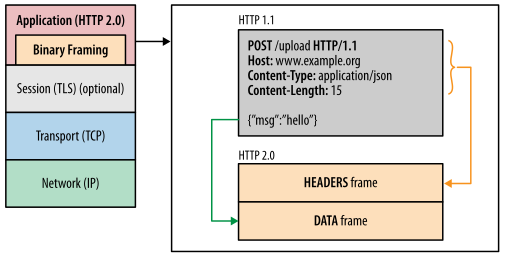
\includegraphics[scale=1.0]{\ImgPath/rys/ramka.png}
\end{center}
	\caption{Schemat ramki protokołu HTTP/2 (źródło: \cite{http2Fundamentals})}
	\label{schematRamki}
\end{figure}
Jest to rozwiązanie dużo bardziej kompaktowe i łatwiejsze w implementacji, niż przesyłanie zwykłego tekstu.
Dzięki temu zabiegowi w ramach jednego połączenia TCP z serwerem może zostać utworzonych wiele dwukierunkowych strumieni danych przesyłających wiadomości HTTP.
Taka wiadomość to w rzeczywistości zapytanie od klienta lub odpowiedź serwera składające się z ramek.
Każda ramka natomiast musi posiadać przynajmniej nagłówek z informacją, do którego strumienia danych należy.
Kodowanie binarne nie ma wpływu na składnię zawartości ramki -- wszystkie nagłówki czy zapytania HTTP/1.1 pozostawiono bez zmian.

\section{Multiplexing}
\label{sectionMultiplexing}
W poprzedniej wersji protokołu, pomimo, że istniała możliwość przesyłania wielu zapytań w ramach jednego połączenia, nie można było wykonywać ich równolegle.
Każde zapytanie musiało być rozpatrywane i odesłane przez serwer do klienta zgodnie z kolejnością nadania, co powodowało efekt head-of-line blocking (problem polegający na head-of-line blocking, dokładniej opisany w \cite{hol}).
Aby wykonywać zapytania równolegle należało utworzyć kilka zapytań TCP, co obciążało serwer oraz było czasochłonne.
Protokół HTTP/2 umożliwia przesyłanie oraz odbieranie wielu wiadomości jednocześnie, co pokazuje schemat na rysunku \ref{schematMultiplexing}.
\begin{figure}[!htbp]
	\begin{center}
\centering
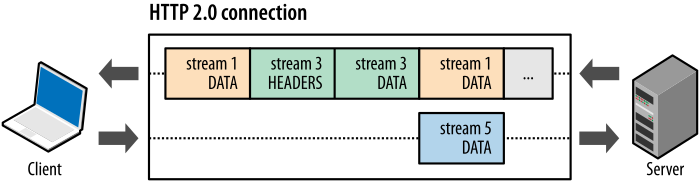
\includegraphics[scale=0.6]{\ImgPath/rys/multiplexing.png}
\end{center}
	\caption{Schemat wykorzystania multiplexingu w HTTP/2 (źródło: \cite{http2Fundamentals})}
	\label{schematMultiplexing}
\end{figure}
Są one rozbijane na pojedyncze ramki, przesyłane, a następnie odczytywane i składane z powrotem w całość po stronie odbiorcy.
Dzięki temu nie jest już konieczne uciekanie się do takich zabiegów jak:
\begin{itemize}
	\item scalanie plików (na przykład webpack),
	\item  wykorzystywanie duszków CSS (więcej o użyciu duszków CSS w kontekście aplikacji internetowych: \cite{sprites}),
	\item domain sharding -- rozdzielanie zasobów strony internetowej na wiele domen.
	Dzięki temu klient może jednocześnie pobierać większą liczbę zasobów, ponieważ liczba aktywnych połączeń z jedną domeną jest ograniczona.
	Zazwyczaj wykorzystywane do pobierania zewnętrznych bibliotek takich jak na przykład jQuery czy Bootstrap (dla zainteresowanych: \cite{domainSharding}).
\end{itemize}
To wszystko sprawia, że aplikacje stają się szybsze oraz prostsze.

\section{Pierwszeństwo}

Po przeczytaniu poprzedniej sekcji możemy dojść do wniosku, że multiplexing nie ma prawa działać, bo przecież zazwyczaj kolejność otrzymanych informacji jednak ma znaczenie.
Z tego powodu HTTP/2 wprowadza system wag zapytań.
Umożliwia on:
\begin{enumerate}
	\item przypisanie wagi w postaci liczby naturalnej od 1 do 256 każdemu strumieniowi danych,
	\item ustalenie zależności danego strumienia od innych.
\end{enumerate}

Informacja o pierwszeństwie umieszczana jest jako odpowiednie pola w nagłówku strumienia.
Gdy zajdzie potrzeba zmiany priorytetów możemy wysłać również odpowiednią ramkę, która zawiera jedynie informacje o pierwszeństwie danego strumienia.
W obu przypadkach przekazujemy informacje o zależności danego strumienia od innych strumieni oraz o jego wadze.
W wypadku, gdy klient nie ustawi tych wartości, to rodzicem strumienia staje się nieistniejący strumień 0 (0x0).
Zostaje on jednocześnie korzeniem drzewa zależności strumieni, od którego zaczynamy rozpatrywanie wszystkich strumieni.
Standardowa waga pakietu, w przypadku, gdy nie została ustalona ta wartość, to 16.
Jeżeli dwa strumienie posiadają tego samego rodzica, to serwer dokonuje podziału zasobów (procesor, pamięć) proporcjonalnie do wag odpowiednich strumieni.
Po przeprocesowaniu strumienia i przygotowaniu odpowiedzi przepustowość pasma również jest proporcjonalna do wagi przypisanej zapytaniu.

Dzięki temu zabiegowi serwer potrafi rozdysponować zasoby (np. CPU czy pamięć) tak, aby w optymalny sposób wykonać prośby nadesłane przez klienta.

\section{Server push}
\label{sectionServerPush}

Wykorzystując protokół HTTP/1.1 nie mamy możliwości otrzymania zasobu, o który nie poprosiliśmy wysyłając zapytanie.
Powoduje to opóźnienia na przykład podczas ładowania strony internetowej.
Zanim otrzymamy skrypty czy arkusze stylów, które wykorzystuje nasza strona musi ona o nie poprosić.
Zapytanie do serwera wysyłane jest gdy w kodzie pliku HTML napotkamy na taki kod (przykład z mojego projektu \ref{push}):
\begin{lstlisting}[caption=Zasoby przesyłane z wykorzystaniem server push, label=push]
<link rel="stylesheet"
	  href="libs/bootstrap/dist/css/bootstrap.min.css">
<link rel="stylesheet"
      href="libs/font-awesome/css/font-awesome.min.css">

<script src="libs/angular/angular.min.js"></script>
\end{lstlisting}
Takie rozwiązanie, chociaż w wielu przypadkach jest pożądane, tutaj jedynie spowalnia działanie aplikacji.
Jeżeli mamy pewność, że użytkownik będzie potrzebował danych zasobów \ref{schematPush} możemy mu je od razu udostępnić, co zdecydowanie skraca czas ładowania aplikacji i dzięki temu unikam niechcianego efektu, gdy strona się załaduje, ale na przykład bez pliku zawierającego style, który jest dopiero przesyłany.
\begin{figure}[!htbp]
	\begin{center}
\centering
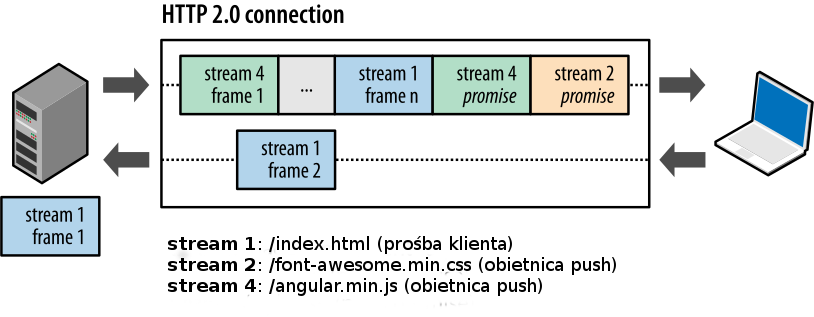
\includegraphics[scale=0.6]{\ImgPath/rys/push.png}
\end{center}
	\caption{Schemat Server push HTTP/2 (źródło: \cite{http2Fundamentals})}
	\label{schematPush}
\end{figure}

\section{Kompresja nagłówków}

Kolejną ważną, chociaż pozornie niezauważalną zmianą jest kompresja nagłówków.
Pomimo, że problem może wydawać się marginalny, to te kilka bajtów w każdym zapytaniu potrafi dość mocno wydłużyć czas komunikacji z serwerem.
HTTP/2 wykorzystuje format kompresji zwany HPACK (opis stndardu: \cite{hpack}), który dzięki wykorzystaniu dwóch technik -- kodowania oraz indeksowania, jest w stanie znacznie usprawnić komunikację ze względu na nagłówki.
Po pierwsze kodowanie Huffmana znacznie kompresuje przesyłane dane.
Dodatkowo klient oraz serwer przechowują listę widzianych wcześniej nagłówków i nie ma potrzeby wysyłania za każdym razem całego nagłówka.
Przesyłamy jedynie pola, które się zmieniły (patrz rysunek \ref{schematHeaderComp}).

\begin{figure}[!htbp]
	\begin{center}
\centering
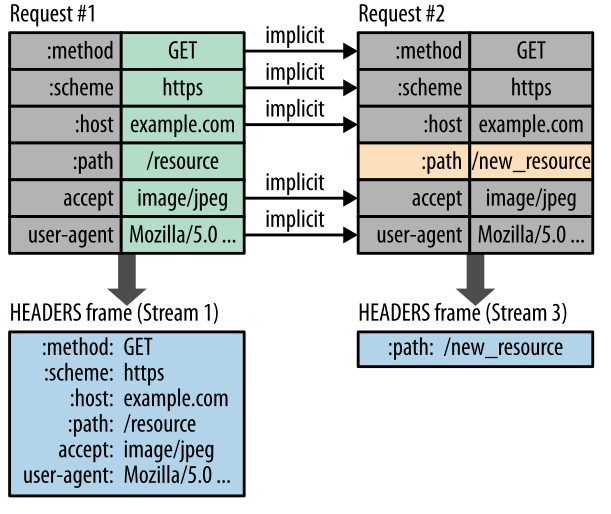
\includegraphics[scale=0.6]{\ImgPath/rys/headercomp.png}
\end{center}
	\caption{Kompresja nagłówków w HTTP/2 (źródło: \cite{http2Fundamentals})}
	\label{schematHeaderComp}
\end{figure}

W powyższych akapitach opisałem techniki wprowadzone w HTTP/2.
W swojej pracy wykorzystam je do zbudowania własnej aplikacji.
Następnie, wykorzystując stworzoną aplikację, zamierzam zbadać wydajność oraz poprawność ich działania. 

\chapter{Budowa aplikacji testowej}

% \section{Struktura aplikacji}
\section{node-spdy -- konfiguracja serwera}

Najważniejszym elementem aplikacji jest konfiguracja serwera, który będzie w stanie obsłużyć zapytania HTTP/2.
Jak pokazuje listing \ref{server} na początku należy ustawić opcje naszego serwera:

\begin{enumerate}
	\item \texttt{plain} -- jeśli opcja jest ustawiona na \texttt{true}, to serwer wykorzystuje protokół HTTP/1.1, 
	\item \texttt{ssl} -- ustawienia zabezpieczeń połączenia -- jeżeli ustawione na \texttt{false} oraz opcja \texttt{plain} ustawiona na \texttt{true}, to serwer będzie wykorzystywał HTTP/1.1 bez zabezpieczania połączenia za pomocą SSL,
	\item \texttt{protocols} -- lista protokołów, z których możemy korzystać,
	\item \texttt{key} -- klucz prywatny do połączeń SSL,
	\item \texttt{cert} -- certyfikat serwera do połączenia SSL.
\end{enumerate}

Następnie uruchamiamy nasz serwer HTTP za pomocą polecenia createServer i podajemy mu naszą konfigurację oraz informację o tym, jak ma się zachować, gdy otrzyma zapytanie od klienta.
W tym wypadku jest to moja aplikacja, więc za każdym razem, gdy serwer otrzyma zapytanie, będzie korzystał ze stworzonych przeze mnie funkcji.

Na koniec musimy ustawić nasz serwer tak, aby nasz serwer nasłuchiwał przychodzących połączeń.
Osiągniemy to przy pomocy funkcji \texttt{listen()}, do której przekazujemy port, na którym nasza aplikacja ma działać.
Jeśli wszystko zakończy się pomyślnie otrzymamy informację o tym, że aplikacja działa na wybranym przez nas porcie.
Jeśli nie, to zostanie zwrócony komunikat o błędzie.

\begin{lstlisting}[caption=Konfiguracja serwera, label=server]
var spdy           = require('spdy');
var port           = 8080;
var fs             = require('fs');
var app            = express();
	
const options = {
  spdy: {
    plain: true,
    ssl: false,
    protocols: ['h2', 'http/1.1'],
  },
  key: fs.readFileSync(__dirname + '/server.key'),
  cert: fs.readFileSync(__dirname + '/server.crt')
};

spdy
  .createServer(options, app)
  .listen(port, (error) => {
    if (error) {
      console.error(error);
      return process.exit(1);
    } else {
      console.log('Listening on port ' + port + '.');
    }
  });
\end{lstlisting}

Jak widać podstawowa konfiguracja serwera HTTP/2 z wykorzystaniem biblioteki node-spdy \cite{spdy} jest dość prostym zadaniem.
Należy jedynie pamiętać o wszystkich ustawieniach oraz wygenerowaniu kluczy dla połączenia SSL, ponieważ bez konfiguracji serwer się nie uruchomi.

\section{Server Push}

Najbardziej wymagającą częścią projektu było zaimplementowanie funkcji server push.
Ostatecznie udało się stworzyć podstronę, która do pełnego działania wymaga biblioteki jQuery.
Normalnie biblioteka ta byłaby wysłana dopiero po odczytaniu pliku push.html przez klienta i wysłaniu zapytania z prośbą o przesłanie jQuery.
Jest to rozwiązanie, w którym tracimy czas na wysłanie zapytania o zasób, który mógł być wysłany od razu.
Server Push zaimplementowany w HTTP/2 daje nam taką możliwość.

Przy pomocy listingu \ref{push} postaram się przybliżyć sposób, w jaki udało mi się zaimplementować tę funkcję.

Najpierw tworzymy routing dla ścieżki \texttt{/push}.
W nim, w zależności od tego co chcemy przesłać, scenariusz będzie trochę inny.
W moim przypadku przesyłam zawartość strony w postaci kodu HTML oraz bibliotekę jquery.
Najpierw wczytujemy plik i zapisujemy jego zawartość.
Jeśli wszystko zostało wykonane pomyślnie, to zapisujemy zawartość pliku HTML do wysłania jako odpowiedź na zapytanie użytkownika.
Następnie wczytujemy zawartość pliku z biblioteką jQuery i umieszczamy ją w strumieniu danych wysyłanym w ramach funkcji Push.
Ustawiamy nagłówki symulowanej prośby, typ odpowiedzi oraz dołączamy zawartość pliku, którą chcemy przesłać.
Zamykamy strumień danych i kończymy odpowiedź komendą res.end().
Oczywiście w ramach jednego zapytania możemy przesłać wiele zasobów.
Tworzymy po prostu kolejne strumienie danych analogicznie do pierwszego, który jest przedstawiony poniżej.

Server Push pomimo ogromnych usprawnień, których wyniki przybliżę w rozdziale \ref{pushSection},
W związku z tym, że klient nie prosił o dane zasoby musimy koniecznie wypełnić nagłówek przesyłanego zasobu, aby przeglądarka mogła odpowiednio zareagować na odebrany zasób.
Na przykład po prostu go odrzucić, gdy znajduje się on już w pamięci podręcznej.
Jest to rozwiązane za pomocą PUSH\textunderscore PROMISE, które jest wysyłane do klienta przed faktycznym przesłaniem całego strumienia.
Jeśli klient zechce, to może odrzucić dany strumień wysyłając ramkę RST\textunderscore STREAM.

\begin{lstlisting}[caption=Konfiguracja server push, label=push]
app.get('/push', function(req, res) {
  fs.readFile('/push.html', function read(err, data) {
    if(err) {
      throw err;
    }
    content = data;
    res.write(content)
  })

  fs.readFile('/jquery.js', function read(err, data) {
    if(err) {
      throw err;
    }
    content = data;
    var stream = res.push('/libs/jquery/dist/jquery.js', {
      status: 200, // optional
      method: 'GET', // optional
      request: { accept: '*/*' },
      response: { 'content-type': 'application/javascript' }
    })
    stream.on('error', function(err) {
      console.log(err);
    })
    stream.end(content)
    res.end();
  })
})
\end{lstlisting}

Na rysunku \ref{schematNoPushDetails} widzimy przykład zapytania bez wykorzystania server push.
Znajdują się tutaj typowe informacje zapytania HTTP:
\begin{enumerate}
	\item sekcja \texttt{Connection Setup} dotycząca ustanowienia połączenia:
	\begin{enumerate}
		\item \texttt{Queueing} -- pakiet zostaje zakolejkowany, jeżeli jest zapytanie o wyższym priorytecie lub osiągnięto maksymalną liczbę połączeń TCP dla jednego klienta (możemy mieć otwartych jednocześnie 6 połączeń TCP),
		\item \texttt{Stalled} -- czas na jaki pakiet utknął z któregoś z powodów wymienionych wyżej,
	\end{enumerate}
	\item sekcja \texttt{Request/Response} dotycząca czasów przesyłania danych:
	\begin{enumerate}
		\item \texttt{Request sent} -- czas wysyłania zapytania,
		\item \texttt{Waiting (TTFB)} -- \texttt{Time To First Byte} jest to czas oczekiwania na otrzymanie pierwszego bajtu odpowiedzi wysłanej przez serwer,
		\item \texttt{Content Download} -- czas pobierania odpowiedzi przez przeglądarkę.
	\end{enumerate}
\end{enumerate}
Natomiast na rysunku \ref{schematPushDetails} nie ma informacji świadczących o tym, że zostało wysłane jakiekolwiek zapytanie -- \texttt{Request sent}, \texttt{Waiting (TTFB)} i \texttt{Content Download}.
Z tego wynika, że klient nie wysłał prośby o dany plik, a mimo to został on wysłany.
Dodatkowym potwierdzeniem, że korzystamy z server push jest informacja, że inicjatorem zapytania jest \texttt{Push/push:4} widoczna w kolumnie \texttt{Initiator}.
Widać też, że czas zapytania to prawie 3 razy mniej (32.34 ms zamiast 12.01 ms) dla danych przesłanych z wykorzystaniem możliwości HTTP/2.
Widać tutaj jak dużo czasu trwa oczekiwanie na zasoby, które mogłyby zostać wysłane od razu.

\begin{figure}[!htbp]
	\begin{center}
\centering
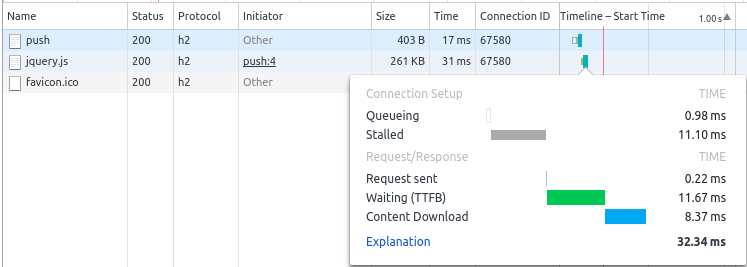
\includegraphics[scale=0.6]{\ImgPath/rys/noPushDetails.png}
\end{center}
	\caption{Szczegóły zapytania wysłanego bez wykorzystania Server Push}
	\label{schematNoPushDetails}
\end{figure}

\begin{figure}[!htbp]
	\begin{center}
\centering
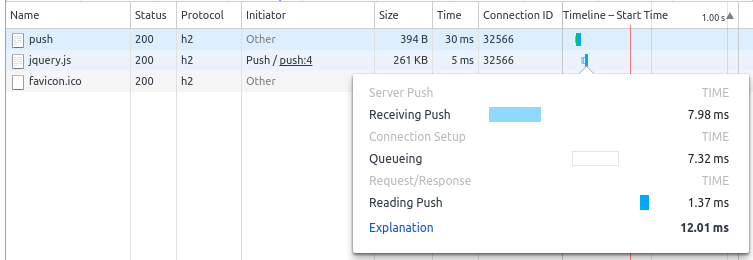
\includegraphics[scale=0.6]{\ImgPath/rys/pushDetails.png}
\end{center}
	\caption{Szczegóły zapytania wysłanego z wykorzystaniem Server Push}
	\label{schematPushDetails}
\end{figure}

\chapter{Testy}

\section{Chrome DevTools}

Do pomiaru prędkości oraz uzyskania innych ważnych informacji wykorzystałem narzędzie Chrome DevTools (więcej informacji o tym narzędziu \cite{devtools}).
Opiszę tutaj pokrótce co i jak mierzyłem za pomocą tego oprogramowania.

Po uruchomieniu konsoli przeglądarki przechodzimy do zakładki Network i naszym oczom ukazuje się okno jak na rysunku \ref{schematDevops}.

\begin{figure}[!htbp]
	\begin{center}
\centering
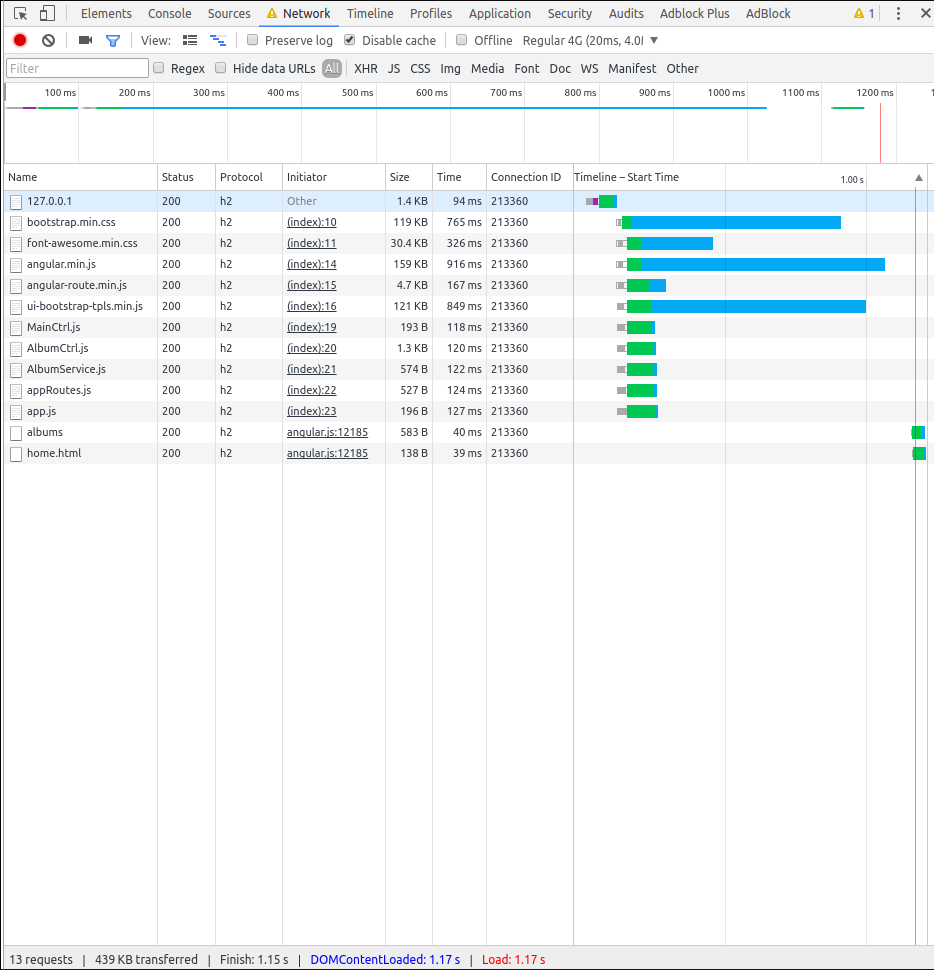
\includegraphics[scale=0.6]{\ImgPath/rys/devops.png}
\end{center}
	\caption{Wygląd okna Chrome DevTools}
	\label{schematDevops}
\end{figure}

Widoczne okno składa się z pięciu głównych elementów:
\begin{enumerate}
	\item paska kontroli -- umożliwia on między innymi edycję wyglądu panelu sieciowego,
	\item paska filtrów -- pozwala na stworzenie reguł i wybór tylko tych pakietów, które nas interesują,
	\item paska przeglądu -- ukazuje nam oś czasu, która daje nam obraz tego, jak przesyłane były pakiety danych,
	\item tabeli zapytań -- zawiera szczegółowe informacje na temat każdego zapytania
	\item podsumowania -- zawiera informacje o łącznej liczbie zapytań, przesłanych danych oraz czasie trwania.
\end{enumerate}

W moich badaniach najczęściej korzystałem z informacji zawartych w tabeli zapytań, a szczególnie z przedstawionej w niej osi czasu.
Po najechaniu kursorem na którykolwiek pasek na osi otrzymujemy szczegółowe informacje o czasie każdego z etapów zapytania jak na rysunku \ref{schematResourceTiming}.

\begin{figure}[!htbp]
	\begin{center}
\centering
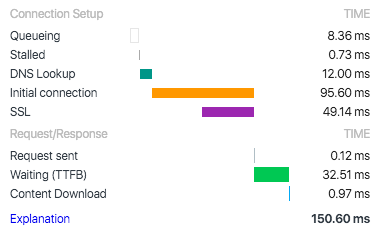
\includegraphics[scale=0.6]{\ImgPath/rys/resource-timing-data.png}
\end{center}
	\caption{Szczegółowe informacje na temat czasu zapytania}
	\label{schematResourceTiming}
\end{figure}

\section{Środowisko testowe}

Aplikacja, którą stworzyłem nosi nazwę LubimySłuchać. 
Jest to aplikacja, w której użytkownik może zarządzać swoją wirtualną kolekcją albumów muzycznych.
W obecnym stadium aplikacja pozwala na:
\begin{enumerate}
	\item przeglądanie listy albumów,
	\item wyszukiwanie albumu po nazwie lub wykonawcy,
	\item dodanie albumu,
	\item edycję albumu,
	\item usunięcie albumu.
\end{enumerate}
Są to podstawowe funkcje, dzięki którym mogłem przetestować protokół HTTP/2. W przyszłości planuję rozwój aplikacji.

Na rysunku \ref{aplikacjaMain} widzimy główny widok mojej aplikacji.
Na górze znajduje się pasek nawigacyjny, po jego prawej stronie jest okno wyszukiwania albumów.
W głónej części mamy podgląd wszystkich dodanych przez użytkownika albumów oraz formularz umożliwiający dodanie kolejnej pozycji do listy.
\begin{figure}[!htbp]
	\begin{center}
\centering
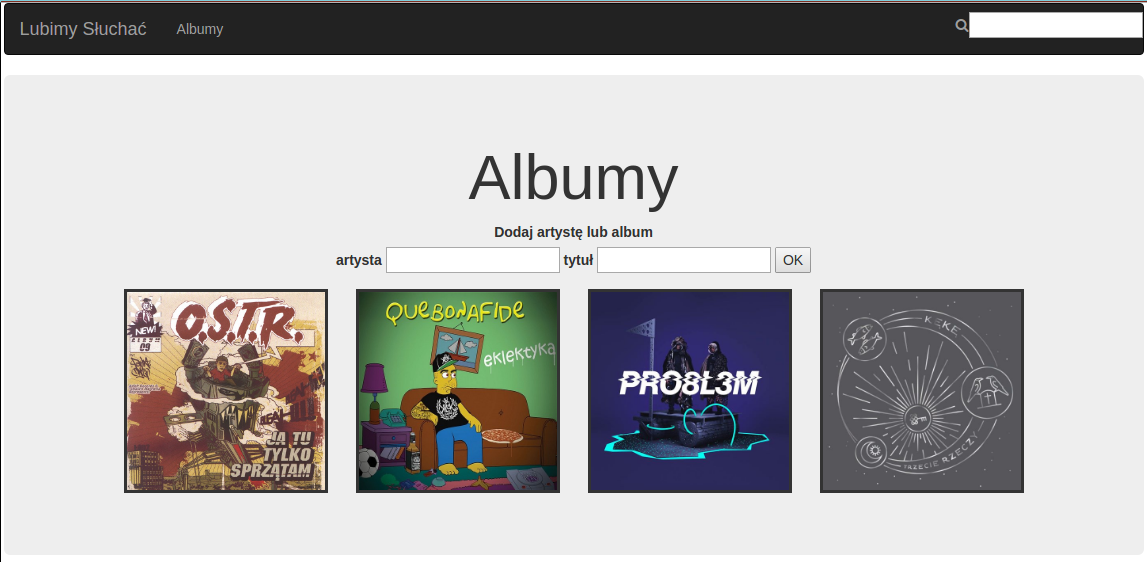
\includegraphics[scale=0.4]{\ImgPath/rys/aplikacjaMain.png}
\end{center}
	\caption{Główne okno aplikacji LubimySłuchać}
	\label{aplikacjaMain}
\end{figure}

Po wpisaniu w okno wyszukiwarki nazwy albumu lub wykonawcy lista jest odpowiednio filtrowana i wyświetlane są tylko pasujące albumy.
Jak widać na rysunku \ref{aplikacjaSearch} wystarczy wpisać fragment nazwy, a aplikacje dynamicznie filtruje listę albumów.

\begin{figure}[!htbp]
	\begin{center}
\centering
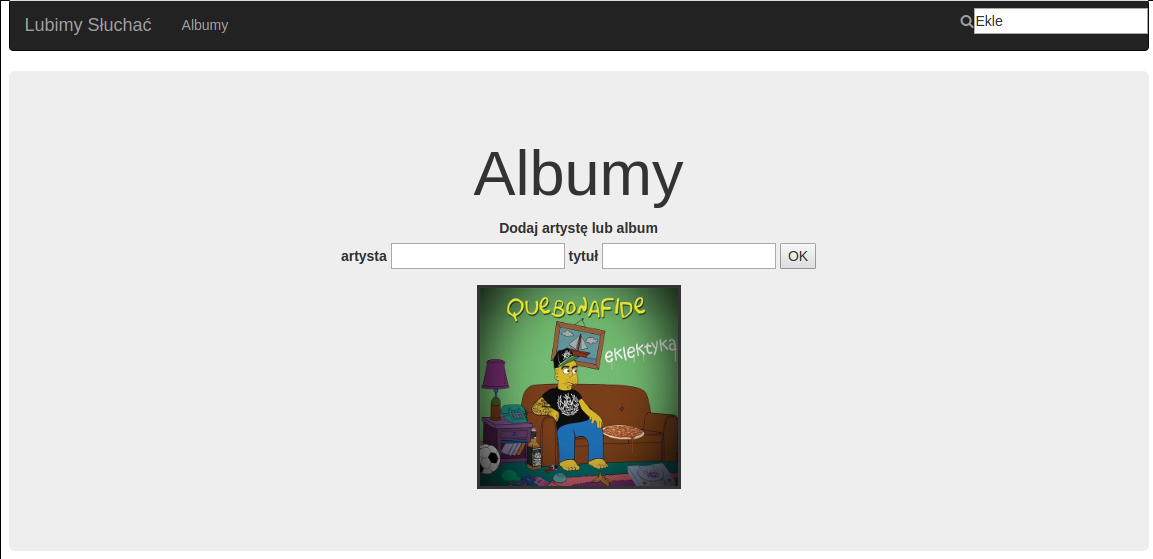
\includegraphics[scale=0.4]{\ImgPath/rys/aplikacjaSearch.png}
\end{center}
	\caption{Widok listy albumów po wprowadzeniu fragmentu nazwy poszukiwanego albumu}
	\label{aplikacjaSearch}
\end{figure}

Takie dynamiczne wyszukiwanie jest możliwe do realizacji w bardzo prosty sposób, dzięki funkcjom udostępnianym przez framework AngularJS.
Na listingu \ref{filter1} widzimy kod pola \texttt{input} odpowiedzialnego za filtrowanie albumów.
Tekst wprowadzony w to pole jest automatycznie przypisywane zmiennej \texttt{searchAlbum}.
Na listingu \ref{filter2} widzimy, że zmienna ta jest wykorzystywana do filtrowania wszystkich albumów: \texttt{ng-repeat="album in albums | filter:searchText"} -- ten fragment jest odpowiedzialny za wyświetlanie kolejnych albumów pobranych z serwera, które spełniają kryteria wyszukiwania.

\begin{lstlisting}[caption=Kod filtra w pasku nawigacyjnym aplikacji, label=filter1]
<ul class="nav navbar-form navbar-right">
  <li>
    <i class="fa fa-search"></i><input ng-model="searchAlbum">
  </li>
</ul>
\end{lstlisting}
\begin{lstlisting}[caption=Kod odpowiedzialny za wyświetlanie albumów, label=filter2]
<div class="box2" ng-repeat="album in albums | filter:searchText"
     ng-mouseenter="active=true"
     ng-mouseleave="active=false"
     ng-click="editWindow=!editWindow">
      <div class="content">
        <p>{{album.artist}}</p>
        <p>{{album.title}}</p>
        <i class="fa fa-trash" aria-hidden="true" ng-show="active" ng-click="deleteAlbum(album._id)"></i>
        <i class="fa fa-pencil" aria-hidden="true" ng-show="active" ng-click="editAlbum(album)"></i>
      </div>
      <img ng-src="/img/{{album.artist}}.jpg"/>
</div>
\end{lstlisting}

Użytkownik ma możliwość dodania, edycji oraz usunięcia albumu ze swojej listy.
Aby dodać album wystarczy wprowadzić artystę oraz tytuł albumu i zostanie on automatycznie dodany po kliknięciu przycisku OK.
PO naciśnięciu przycisku OK wywoływana jest funkcja widoczna na listingu \ref{add1}.
Jest ona odpowiedzialna za przkazanie informacji dotyczących albumu do serwera, a następnie za odczytanie odpowiedzi serwera i poinformowanie użytkownika czy operacja się udała.
Funkcja wywoływana po stronie serwera, która jest widoczna na listingu \ref{add2}, tworzy nowy album oraz przypisuje mu konkretne wartości otrzymane od użytkownika i wysyła komunikat o tym, czy operacja się powiodła.

\begin{lstlisting}[caption=Kod odpowiedzialny za wysłanie zapytania do serwera z prośbą o dodanie albumu, label=add1]
  $scope.addAlbum = function(newAlbum) {
    $http.post('/api/album', {'artist': newAlbum.artist,
                              'title': newAlbum.title})
      .success(function() {
        $scope.newAlbum = {};
        $scope.getAlbums();
        alert('Dodano album!');
      }).
      error(function(err) {
        console.log(err);
      });
  };
\end{lstlisting}


\begin{lstlisting}[caption=Kod odpowiedzialny za dodanie albumu do bazy, label=add2]
app.post('/api/album', function(req, res) {
  album = new Album();
  album.title = req.body.title;
  album.artist = req.body.artist;

  album.save(function(err) {
    if (err) res.send(err);
    res.json({message: 'Album created!'});
    })
});
\end{lstlisting}

O sukcesie operacji zostaniemy poinformowani stosownym komunikatem widocznym na rysunku \ref{aplikacjaAdd}.

\begin{figure}[!htbp]
	\begin{center}
\centering
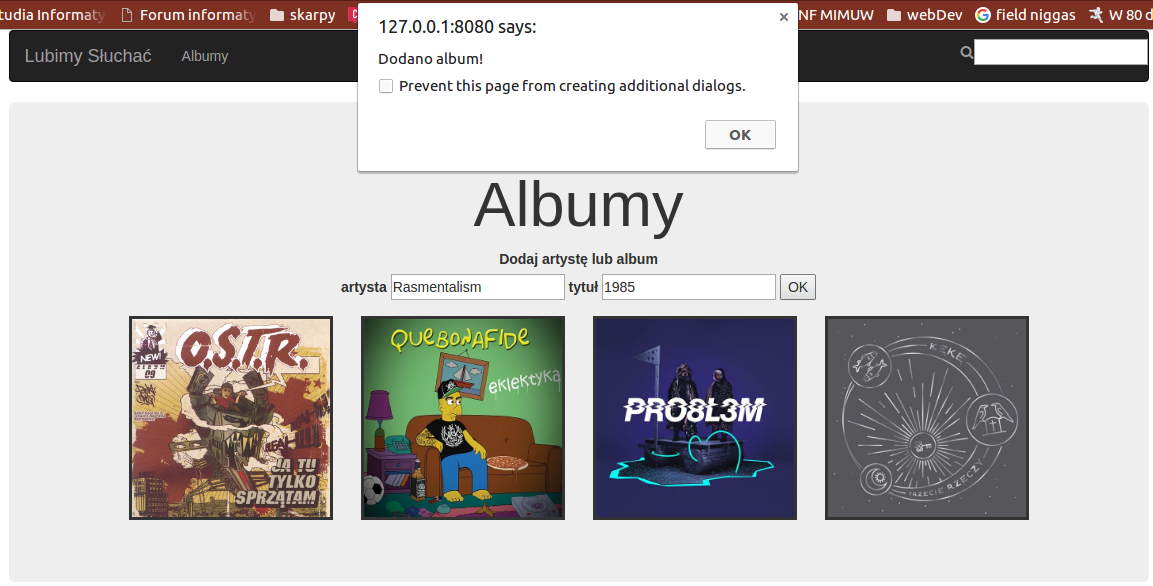
\includegraphics[scale=0.4]{\ImgPath/rys/aplikacjaAdd.png}
\end{center}
	\caption{Widok aplikacji po wprowadzeniu danych nowego albumu i kliknięciu przycisku OK}
	\label{aplikacjaAdd}
\end{figure}

Jak widać na rysunku \ref{aplikacjaAdded} album natychmiast pojawia się na liście.

\begin{figure}[!htbp]
	\begin{center}
\centering
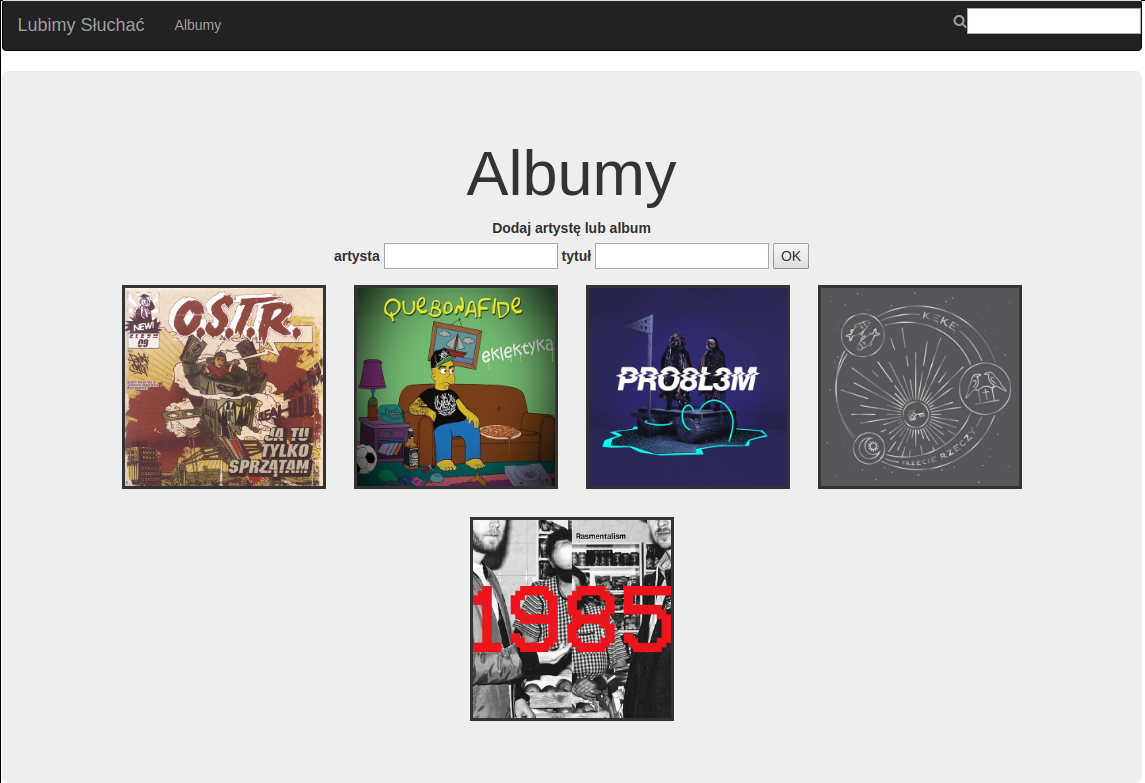
\includegraphics[scale=0.4]{\ImgPath/rys/aplikacjaAdded.png}
\end{center}
	\caption{Widok aplikacji po udanym dodaniu albumu 1985 zespołu Rasmentalism}
	\label{aplikacjaAdded}
\end{figure}

Użytkownik ma również możliwość edycji oraz usunięcia wybranego albumu. Po najechaniu na wybraną okładkę pojawiają się podstawowe informację o nim oraz ikonki usunięcia oraz edycji wpisu. jest to widoczne na rysunku \ref{aplikacjaEdit}.

\begin{figure}[!htbp]
	\begin{center}
\centering
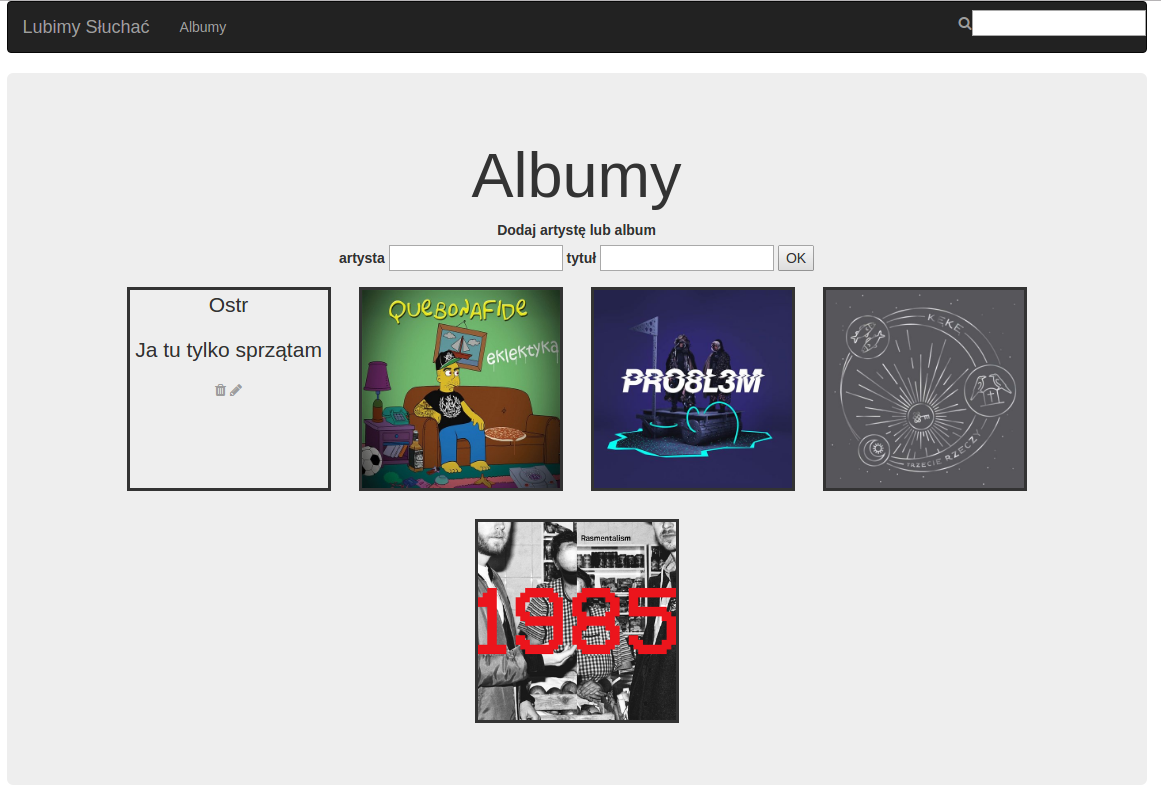
\includegraphics[scale=0.3]{\ImgPath/rys/aplikacjaEdit.png}
\end{center}
	\caption{Widok szczegółów albumu}
	\label{aplikacjaEdit}
\end{figure}

Po kliknięciu na ikonę symbolizującą kosz na śmieci album zostaje usunięty, a aplikacja informuje nas o tym stosownym komunikatem, który widzimy na rysunku \ref{aplikacjaDelete}.
Album natychmiast znika z listy.

\begin{figure}[!htbp]
	\begin{center}
\centering
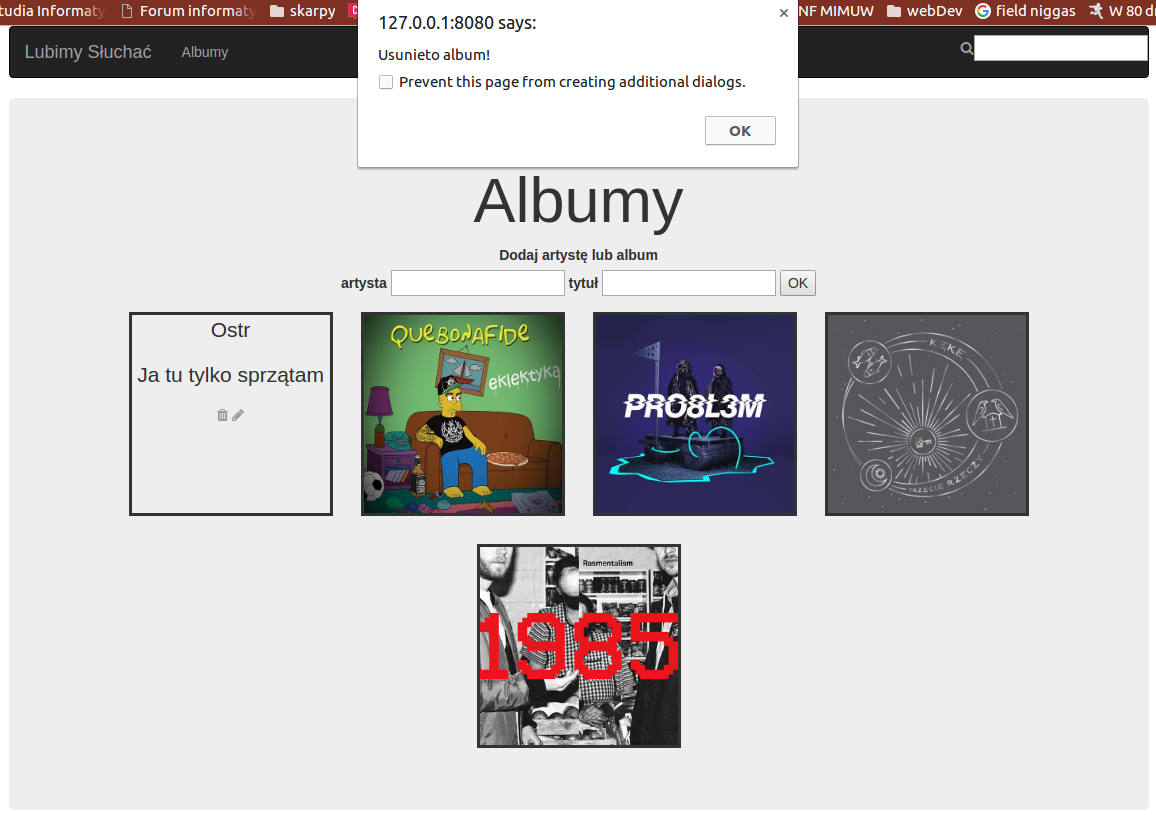
\includegraphics[scale=0.4]{\ImgPath/rys/aplikacjaDelete.png}
\end{center}
	\caption{Widok po naciśnięciu ikonki kosza na śmieci}
	\label{aplikacjaDelete}
\end{figure}

Po naciśnięciu symbolu kosza na śmieci wywoływana jest funkcja odpowiedzialna za usunięcie albumu widoczna na listingu \ref{remove1}. Funkcja przekazuje do serwera numer id albumu, który użytkownik chce usunąć, a następnie oczekuje na wynik działania i zwraca odpowiedni komunikat.

\begin{lstlisting}[caption=Kod odpowiedzialny za przekazania id usuwanego albumu do serwera, label=remove1]
$scope.deleteAlbum = function(id) {
  $http.delete('/api/album/' + id)
    .success(function() {
      $scope.getAlbums();
      alert('Usunieto album!');
    }).
    error(function(err) {
      console.log(err);
    });
};
\end{lstlisting}

Po stronie serwera funkcja, widoczna na listingu \ref{remove2}, która otrzymała numer albumu stara się wyszukać odpowiedni wpis bazując na tym numerze. Jeśli uda się znaleźć dany album, to jest on usuwany, a do klienta zwracany jest odpowiedni komunikat.
\begin{lstlisting}[caption=Kod odpowiedzialny za usunięcie albumu o wybranym id z bazy, label=remove2]
app.delete('/api/album/:id', function(req, res) {
  Album.findById(req.params.id, function(err, album) {
    album.remove(function (err, album) {
      if(err) res.send(err);
      res.json({message: 'Album removed! ' + album.id});
    });
  });
});
\end{lstlisting}
\section{Przygotowanie testów}

Przed przejściem do porównania prędkości działania obu wersji protokołu chciałem zaprezentować pierwsze efekty implementacji protokołu HTTP/2, które przedstawia rysunek \ref{schematWorkingExample}.

\begin{figure}[!htbp]
	\begin{center}
\centering
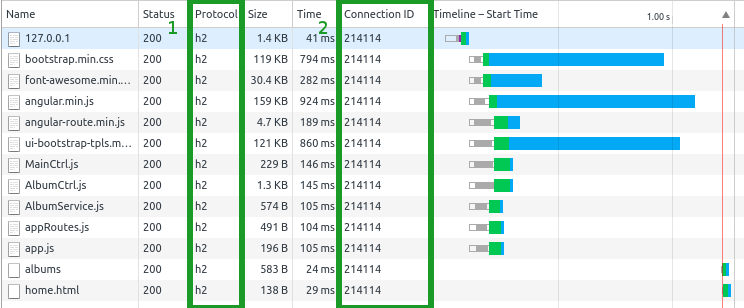
\includegraphics[scale=0.6]{\ImgPath/rys/workingExample.png}
\end{center}
	\caption{Dowód działania protokołu HTTP/2}
	\label{schematWorkingExample}
\end{figure}

Widzimy tutaj dwie rzeczy, które powinny nas zainteresować. W sekcji \texttt{Protocol} oznaczonej na rysunku \ref{schematWorkingExample} numerem 1 widnieje napis h2 przy każdym zapytaniu.
Jest to informacja, że do komunikacji z serwerem wykorzystana została najnowsza wersja protokołu HTTP.
Dodatkowo w sekcji \texttt{Connection ID} (na rysunku \ref{schematWorkingExample} jest to numer 2) widzimy, że wszystkie zapytania zostały wykonane z wykorzystaniem tego samego połączenia TCP.
Nie mogłoby to mieć miejsca, gdybyśmy wykorzystali HTTP/1.1, co pokazuje rysunek \ref{schematWorkingExampleH1}.

\begin{figure}[!htbp]
	\begin{center}
\centering
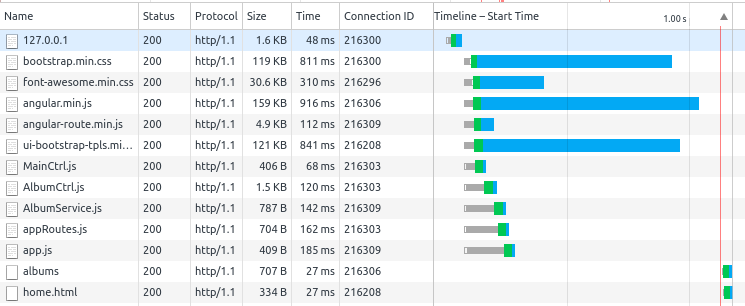
\includegraphics[scale=0.6]{\ImgPath/rys/workingExampleH1.png}
\end{center}
	\caption{Przykładowe linia czasu dla zapytań wykonanych w HTTP/1.1}
	\label{schematWorkingExampleH1}
\end{figure}

Na rysunku widzimy, że protokół z jakiego korzystamy to HTTP/1.1, a wszystkie zapytania, które są wykonywane równolegle przesyłane są w ramach różnych połączeń TCP.
Świadczą o tym wartości w kolumnie 'Connection ID'.

Jeszcze jedną ciekawą rzeczą są wielkości nagłówków.
Dzięki przejściu na kodowanie binarne nagłówki w protokole HTTP/2 są o wiele mniejsze (w moim przykładzie jest to 20 B dla HTTP/2 i 136 B dla HTTP/1.1) niż w tekstowym HTTP/1.1.
W swojej pracy zaimplementowałem możliwość wysłania zapytania, które w odpowiedzi dostaje odpowiedź w postaci samego nagłówka.
Dzięki temu można porównać wielkość nagłówków HTTP na konkretnym przykładzie przedstawionym na listingu \ref{empty}.
Na początku tworzymy nagłówek odpowiedzi ze statusem \texttt{200}, który informuje, że zapytanie powiodło się.
Następnie za pomocą \texttt{res.end('')} tworzymy pustą odpowiedź i odsyłamy wszystko do użytkownika.

\begin{lstlisting}[caption=Wygląd funkcji wykonywanej po wykonaniu zapytania \texttt{GET} na adres \texttt{/empty}, label=empty]
app.get('/empty', function(req, res) {
	res.writeHead(200);
	res.end('');
});
\end{lstlisting}
Wyniki przedstawiają rysunki \ref{schematEmptyRes} i \ref{schematEmptyResH1}.

\begin{figure}[!htbp]
	\begin{center}
\centering
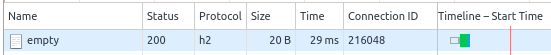
\includegraphics[scale=0.6]{\ImgPath/rys/emptyRes.png}
\end{center}
	\caption{Pusta odpowiedź w HTTP/2}
	\label{schematEmptyRes}
\end{figure}

\begin{figure}[!htbp]
	\begin{center}
\centering
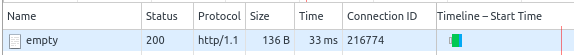
\includegraphics[scale=0.6]{\ImgPath/rys/emptyResH1.png}
\end{center}
	\caption{Pusta odpowiedź w HTTP/1.1}
	\label{schematEmptyResH1}
\end{figure}

Od razu widać, że nagłówki w najnowszej wersji protokołu uległy znacznej kompresji. 

\section{Porównanie prędkości protokołu HTTP/2 i HTTP/1.1}

W ramach tego testu sprawdzałem prędkość ładowania wszystkich zasobów strony z wyłączonym CACHE przeglądarki oraz z ustawioną prędkością Regular 4G (20ms, 4.0 Mb/s, 3.0 Mb/s).
Dane z wykorzystaniem protokołu HTTP/1.1 są przesyłane za pomocą niezabezpieczonego połączenia.
HTTP/2 do utworzenia połączenia wymaga zabezpieczenia SSL.
Taki test nie jest miarodajny, ponieważ czas nawiązania połączenia zabezpieczonego zawsze będzie dłuższy.
Jest to związane ze sposobem nawiązywania bezpiecznego połączenia -- przed rozpoczęciem przesyłania jakichkolwiek informacji serwer musi przesłać do użytkownika certyfikat SSL, który musi zostać zweryfikowany po stronie klienta.
Następnie, jeśli certyfikat jest godny zaufania, klient przesyła odpowiednią informację do serwera.
Sytuację, kiedy korzystamy z zabezpieczonego połączenia HTTP/1.1 przedstawię w następnej sekcji.

\begin{tabular}{c|c|c}
Próba & HTTP/1.1 & HTTP/2 \\ \hline
1 & 1.23s & 1.26s\\
2 & 1.49s & 1.12s\\
3 & 1.28s & 1.39s\\
4 & 1.20s & 1.09s\\
5 & 1.22s & 1.09s\\
6 & 1.25s & 1.26s\\
7 & 1.21s & 1.12s\\
8 & 1.25s & 1.11s\\
9 & 1.21s & 1.16s\\
10 & 1.26s & 1.10s\\ \hline
ŚREDNIA & 1.26s & 1.17s\\
\end{tabular}

Tabela ukazuje wyniki wykonanych pomiarów.
Jak widać protokół HTTP/2 przyśpiesza czas ładowania strony o około 15\%.
W dużej mierze jest to czas zaoszczędzony na nawiązywanie nowych połączeń TCP.
Sporą oszczędność utrzymujemy też dzięki zmniejszeniu objętości nagłówków odpowiedzi.

Na rysunkach \ref{schematBasicTest} oraz \ref{schematBasicTestH1} widoczny jest przykładowy wynik testu.
W sekcji podsumowania widoczna jest całkowita objętość przesłanych danych. Są to odpowiednio 443 KB i 439 KB dla protokołu HTTP/1.1 i HTTP/2,
Możemy też porównać objętości oraz czasy przesyłania poszczególnych plików.

\begin{figure}[!htbp]
	\begin{center}
\centering
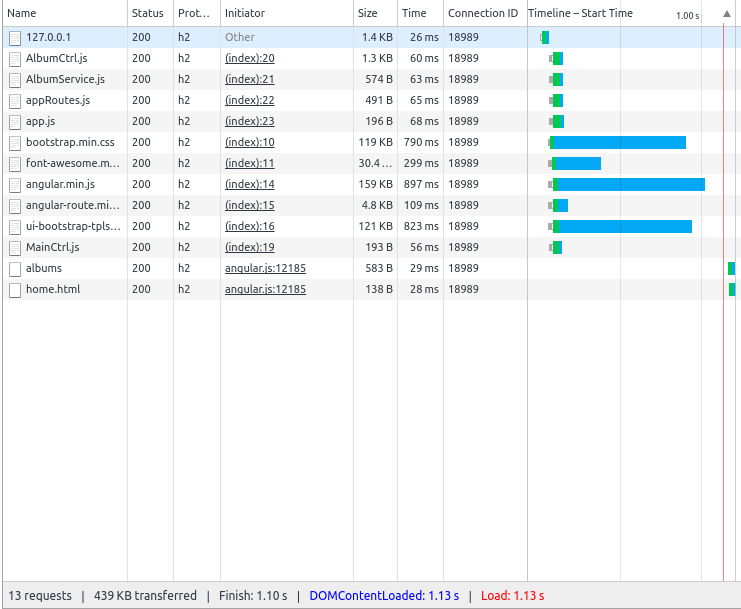
\includegraphics[scale=0.6]{\ImgPath/rys/basicTest.png}
\end{center}
	\caption{Czas ładowania strony dla HTTP/2}
	\label{schematBasicTest}
\end{figure}

\begin{figure}[!htbp]
	\begin{center}
\centering
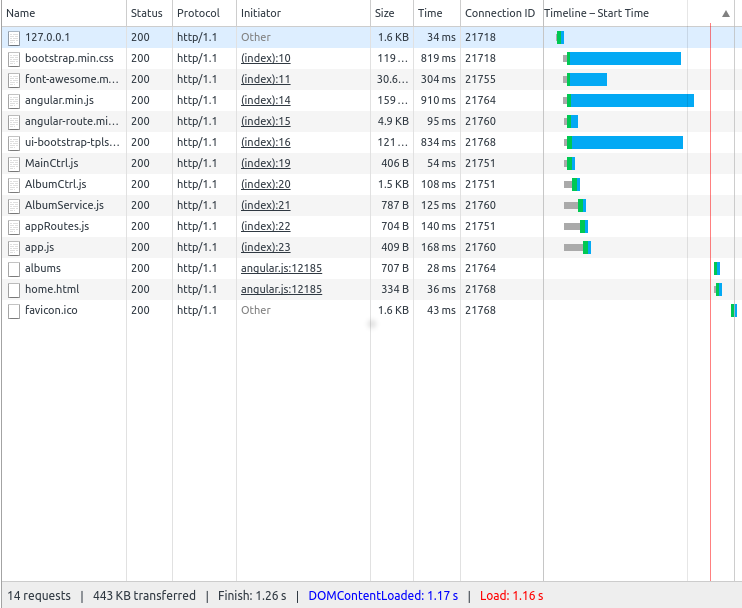
\includegraphics[scale=0.6]{\ImgPath/rys/basicTestH1.png}
\end{center}
	\caption{Czas ładowania strony dla HTTP/1.1 bez SSL}
	\label{schematBasicTestH1}
\end{figure}

Wykres przedstawiony na rysunku \ref{schematTest1} ukazuje porównanie wyników w każdej z prób oraz wynik średni dla obu protokołów.

\begin{figure}[!htbp]
	\begin{center}
\centering
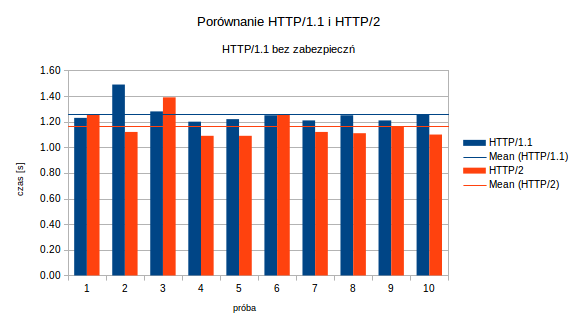
\includegraphics[scale=0.6]{\ImgPath/rys/test1.png}
\end{center}
	\caption{Wykres podsumowujący}
	\label{schematTest1}
\end{figure}

\section{Porównanie prędkości przy bezpiecznym połączeniu HTTP/1.1}

W tym teście dane przesyłane za pomocą protokołu HTTP/1.1 są zabezpieczone SSL.

\begin{tabular}{c|c|c}
Próba & HTTP/1.1 & HTTP/2 \\ \hline
1 & 1.22s & 1.25s \\
2 & 1.49s & 1.29s \\
3 & 1.27s & 1.20s \\
4 & 1.26s & 1.18s \\
5 & 1.27s & 1.17s \\
6 & 1.26s & 1.24s \\
7 & 1.26s & 1.20s \\
8 & 1.26s & 1.23s \\
9 & 1.31s & 1.21s \\
10 & 1.36s & 1.17s\\ \hline
ŚREDNIA & 1.29s & 1.21s \\
\end{tabular}

W powyższym teście protkół HTTP/2 uzyskał wyniki lepsze średnio o 6\%.
Na podstawie tego testu widzimy też, że w przypadku wykorzystania zabezpieczonego połączenia czasy dla HTTP/1.1 są minimalnie większe, niż bez SSL.

Wykres przedstawiony na schemacie \ref{schematTest2} ukazuje porównanie wyników w każdej z prób oraz wynik średni dla obu protokołów.

\begin{figure}[!htbp]
	\begin{center}
\centering
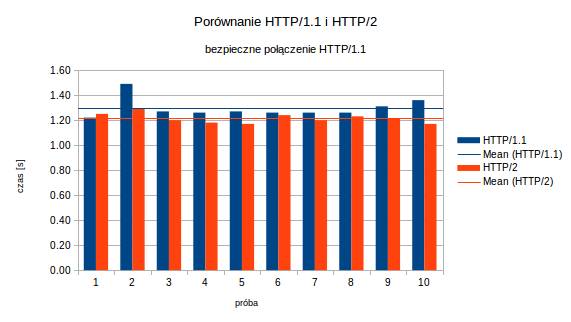
\includegraphics[scale=0.6]{\ImgPath/rys/test2.png}
\end{center}
	\caption{Porównanie czasów pobierania zasobów w kolejnych próbach}
	\label{schematTest2}
\end{figure}

\section{Porównanie prędkości z włączonym CACHE}

\begin{tabular}{c|c|c}
Próba & HTTP/1.1 & HTTP/2 \\ \hline
1 & 709ms & 534ms \\
2 & 555ms & 483ms \\
3 & 622ms & 527ms \\
4 & 625ms & 511ms \\
5 & 550ms & 518ms \\
6 & 546ms & 555ms \\
7 & 603ms & 557ms \\
8 & 517ms & 496ms \\
9 & 584ms & 531ms \\
10 & 521ms & 532ms \\ \hline
ŚREDNIA & 583ms & 524ms \\
\end{tabular}

Kolejny test pokazuje, że średnio czas ładowania strony z wykorzystaniem HTTP/2 jest około 11\% krótszy.
Jak można było się spodziewać czasy z wykorzystaniem pamięci podręcznej przeglądarki będą znacznie mniejsze, niż gdy ta pamięć jest wyłączona.
Pokazuje to jak ważnym elementem pracy twórcy aplikacji internetowych jest rozsądne zarządzanie zasobami, które mogę być przechowywane w pamięci podręcznej po stronie klienta i nie muszą one być za każdym razem wysyłane ponownie.

Obrazują to poniższe rysunki. Na rysunku \ref{schematNoCacheExample} widzimy, co się dzieje, gdy pierwszy raz wchodzimy na daną stronę lub mamy wyłączoną pamięć podręczną przeglądarki.
Czas pobierania niektórych zasobów (niebieska część paska) jest elementem, który zabiera najwięcej czasu.
Natomiast, gdy spojrzymy na rysunek \ref{schematCacheExample}, to praktycznie nie widzimy niebieskiej części paska.
Taka sytuacja ma miejsce, gdy wchodzimy na stronę kolejny raz.
Na rysunku \ref{schematCacheExample} w sekcji \texttt{Status} widzimy status \texttt{304}.
Takim statusem opatrzona jest odpowiedź serwera w wypadku, gdy od czasu ostatniego razu, gdy pobieraliśmy dany zasób nie zmienił się on i nie ma potrzeby jego ponownego wysyłania.
\begin{figure}[!htbp]
	\begin{center}
\centering
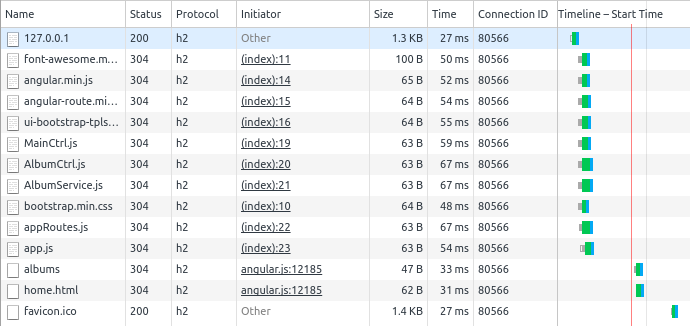
\includegraphics[scale=0.6]{\ImgPath/rys/cacheExample.png}
\end{center}
	\caption{Przykład zapytania z wykorzystaniem kieszeniowania}
	\label{schematCacheExample}
\end{figure}

\begin{figure}[!htbp]
	\begin{center}
\centering
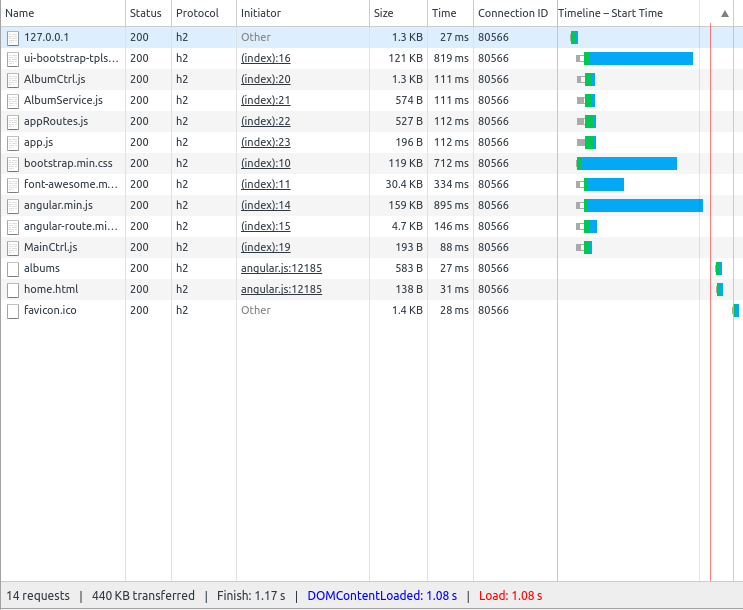
\includegraphics[scale=0.6]{\ImgPath/rys/noCacheExample.png}
\end{center}
	\caption{Przykład zapytania bez wykorzystania kieszeniowania}
	\label{schematNoCacheExample}
\end{figure}

Wykres przedstawiony na schemacie \ref{schematTest3} ukazuje porównanie wyników w każdej z prób oraz wynik średni dla obu protokołów.

\begin{figure}[!htbp]
	\begin{center}
\centering
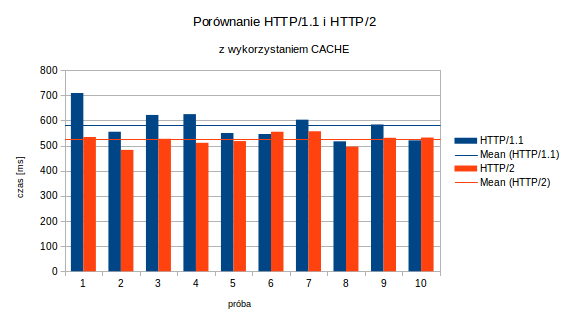
\includegraphics[scale=0.6]{\ImgPath/rys/test3.png}
\end{center}
	\caption{Czasy pobierania zasobów z wykorzystaniem kieszeniowania w kolejnych próbach}
	\label{schematTest3}
\end{figure}

\section{Porównanie prędkości przy wykorzystaniu Server Push}
\label{pushSection}

Ostatni test chciałem przeprowadzić dla zapytania wykorzystującego wprowadzony przez HTTP/2 Server Push, który, z punktu widzenia programisty aplikacji internetowych, wydaje się być najciekawszą nowością wprowadzoną do protokołu HTTP.

\begin{tabular}{c|c|c|c}
Próba & HTTP/1.1 & HTTP/2 & HTTP/2 PUSH \\ \hline
1 & 444ms & 454ms & 387ms \\
2 & 456ms & 441ms & 372ms \\
3 & 386ms & 515ms & 351ms \\
4 & 380ms & 436ms & 471ms \\
5 & 407ms & 342ms & 415ms \\
6 & 404ms & 438ms & 420ms \\
7 & 481ms & 385ms & 470ms \\
8 & 471ms & 450ms & 253ms \\
9 & 567ms & 481ms & 269ms \\
10 & 418ms & 413ms & 409ms \\ \hline
ŚREDNIA & 441ms & 436ms & 382ms \\
\end{tabular}

Poniższe rysunki (\ref{schematNoPushExample11}, \ref{schematNoPushExample} i \ref{schematPushExample}) ukazują porównanie przykładowych zapytań z powyższego testu.

\begin{figure}[!htbp]
	\begin{center}
\centering
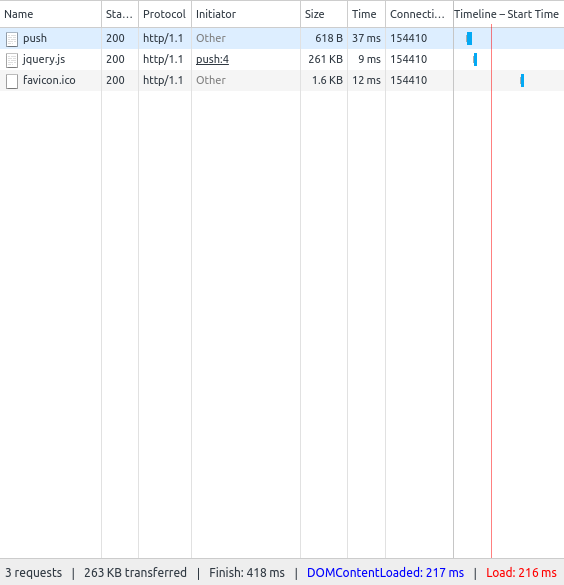
\includegraphics[scale=0.6]{\ImgPath/rys/noPushExample11.png}
\end{center}
	\caption{Przykład zapytania dla HTTP/1.1}
	\label{schematNoPushExample11}
\end{figure}

\begin{figure}[!htbp]
	\begin{center}
\centering
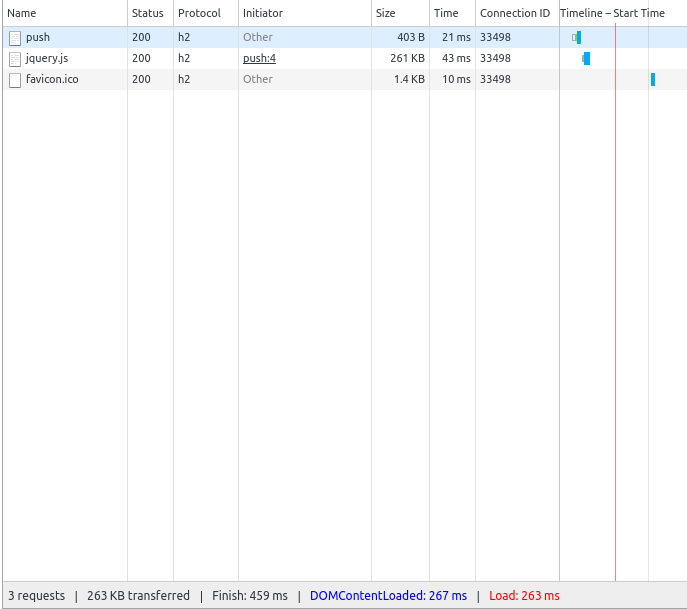
\includegraphics[scale=0.6]{\ImgPath/rys/noPushExample.png}
\end{center}
	\caption{Przykład zapytania bez wykorzystania Server Push}
	\label{schematNoPushExample}
\end{figure}

\begin{figure}[!htbp]
	\begin{center}
\centering
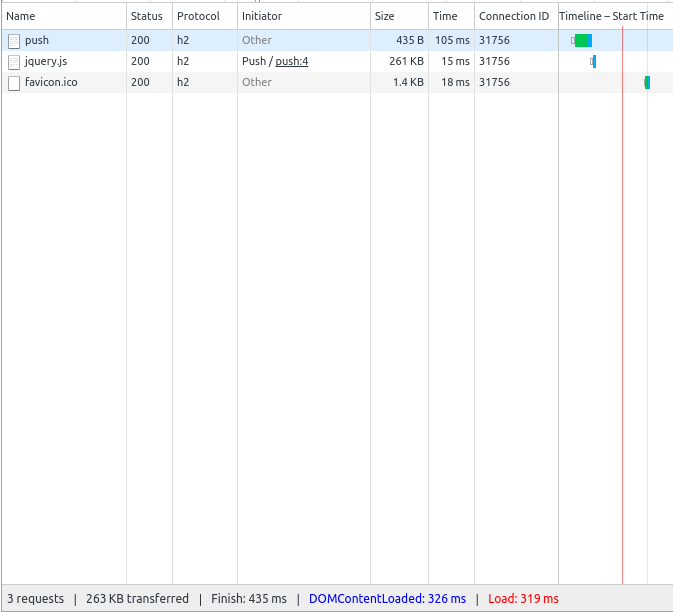
\includegraphics[scale=0.6]{\ImgPath/rys/pushExample.png}
\end{center}
	\caption{Przykład zapytania wykorzystującego Server Push}
	\label{schematPushExample}
\end{figure}

Wykres przedstawiony na schemacie \ref{schematTest4} ukazuje porównanie wyników w każdej z prób oraz wynik średni dla wszystkich przypadków.

\begin{figure}[!htbp]
	\begin{center}
\centering
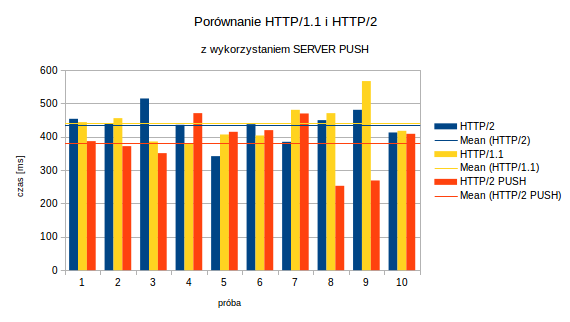
\includegraphics[scale=0.6]{\ImgPath/rys/test4.png}
\end{center}
	\caption{Wykres podsumowujący}
	\label{schematTest4}
\end{figure}

\section{Kompatybilność popularnych przeglądarek internetowych z HTTP/2}

Ważną cechą poza szybkością aplikacji jest również jej niezawodność oraz uniwersalność.
Aby aplikacja była uniwersalna użytkownik musi mieć możliwość jej uruchomienia w różnych środowiskach.
Dlatego przeprowadzięłm testy wsparcia HTTP/2 przez popularne przeglądarki.
Testy przegląderek Firefox, Chrome oraz Opera przeprowadziłem na Ubuntu 16.04.
Mobilną wersję przeglądarki Safari przetestowałem na telefonie iPhone 6 z wersją oprogramowania 10.2.
Testy Edge oraz Internet Explorer zostały przeprowadzone na maszynie wirtualnej z zainstalowanym Windows 8.
Wyniki moich badań przedstawiam w poniższej tabelii.

\begin{tabular}{c|c|c|c|c|c|c}
Lp & Firefox & Chrome & Opera & Safari & Internet Explorer & Edge \\ \hline
1. & \cellcolor{green!50}50 & \cellcolor{green!50}55 & \cellcolor{green!50}42 & & & \cellcolor{green!50}14 \\

2. & \cellcolor{green!50}49 & \cellcolor{green!50}54 & \cellcolor{green!50}41 & \cellcolor{green!50}10.2 & \cellcolor{red!50}11 & \cellcolor{green!50}13 \\

3. & \cellcolor{green!50}48 & \cellcolor{green!50}53 & \cellcolor{green!50}40 & & & \cellcolor{green!50}12 \\
\end{tabular}

Jak widać protokół HTTP/2 jest prawie w pełni wspierany przez najpopularniejsze przeglądarki internetowe w najnowszych wersjach.
Daje nam to pewność, że aplikacja stworzona z wykorzystaniem tej technologii będzie sprawnie działać u większości użytkowników.
Jak widać tylko najnowsza wersja przeglądarki Internet Explorer nie wspiera HTTP/2.
Należy zaznaczyć, że ostatnia aktualizacja IE miała miejsce pod koniec roku 2015, więc nie jest to już wspierany produkt i większość użytkowników odchodzi od niego.

\chapter{Wnioski}

% co jeszcze moglem zrobic
% testy pusha z webpackiem
% testy z poziomu TCP
% testy na wiekszych rzeczach

W obecnych czasach, gdy technologia tak szybko porusza się do przodu, korzystanie z rozwiązań, które nie zmieniły się od ponad 15 latu wydaje się niewłaściwe.
HTTP/1.1 coraz mocniej ogranicza możliwości programistów i nie pozwala rozsądnie i w pełni wykorzystać zasobów, którymi dzisiaj dysponujemy.
Po przeczytaniu, że numer dwa przy wersji protokołu, to właściwie tylko informacja o tym, że nie jest on wstecznie kompatybilny zacząłem się zastanawiać czy nie jest to swego rodzaju uspokojenie pokładanych w tym protokole oczekiwań.
Postanowiłem więc przeprowadzić testy, których wynikiem jest niniejsza praca.

Patrząc na wyniki testów widać przyśpieszenie, względem starszej wersji protokołu.
Pokazuje to, że wprowadzone udoskonalenia mogą w przyszłości przyczynić się do znacznego przyspieszenia aplikacji internetowych.

Dodatkowo protokół HTTP/2 to nie tylko szybkość, ale też jakość połączenia i jego bezpieczeństwo.
Bardzo dobrym krokiem jest wymuszanie na twórcach korzystanie z certyfikatów bezpieczeństwa.
Na pewno sprawi to, że sieć będzie się stawać coraz bezpieczniejszym miejscem i o wiele trudniej będzie przestępcy wykorzystać zwykłego użytkownika.

Wykorzystanie multiplexingu rozwiązało ostatecznie problem HOL blocking, który w niektórych przypadkach potrafił bardzo mocno spowolnić działanie aplikacji. 
Oczywiście były sposoby, żeby sobie z tym poradzić.
Przykładem jest wykorzystywanie wielu połączeń TCP do przesyłania informacji równolegle.
Takie rozwiązanie jednak znacznie bardziej obciąża serwer niepotrzebnymi prośbami o połączenie.
Multiplexing pozwala na przesyłanie wielu informacji w ramach jednego połączenia, a dodatkowo kolejność przesyłanych informacji nie ma znaczenia.

Kolejny element, czyli kompresja nagłówków.
Może nie jest on tak znaczący dla zasobów o bardzo dużej objętości.
Możemy dojść do takiego wniosku na pierwszy rzut oka, jednak podsumowując powtarzającą się część nagłówków, widać, że ma to niemałe przełożenie na ilość przesyłanych danych.

Na koniec chciałem przedstawić wykresy przedstawiające  mediane wyników pierwszych trzech testów (rysunek \ref{schematMedianaTests}) oraz oddzielnie dla ostatniego testu dotyczącego SERVER PUSH (rysunek \ref{schematMedianaTest4}).
Należy pamiętać, że ostatni test został przeprowadzony na innym zestawie pobieranych danych.
Co ciekawe, przeciętna wartość dla testu HTTP/2 bez SERVER PUSH jest niższa, niż z wykorzystaniem tej technologii.

\begin{figure}[!htbp]
	\begin{center}
\centering
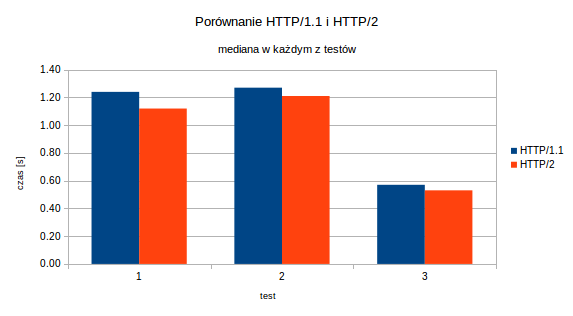
\includegraphics[scale=0.6]{\ImgPath/rys/medianaTests.png}
\end{center}
	\caption{Mediany wyników trzech pierwszych testów}
	\label{schematMedianaTests}
\end{figure}

\begin{figure}[!htbp]
	\begin{center}
\centering
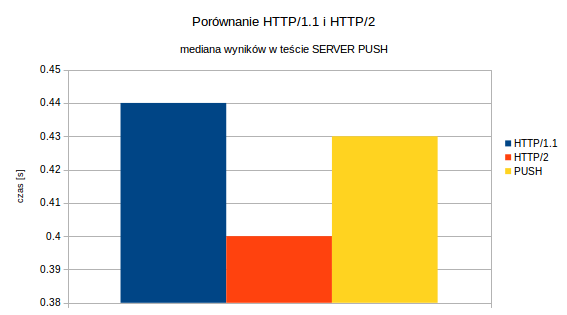
\includegraphics[scale=0.6]{\ImgPath/rys/medianaTest4.png}
\end{center}
	\caption{Mediany wyników testu SERVER PUSH}
	\label{schematMedianaTest4}
\end{figure}

Jak widać, chociaż HTTP/2 jest stosunkowo nową technologią, to jego potencjał w tworzeniu wydajnych aplikacji internetowych jest ogromny. Wyniki moich badań napawają pozytywnie na przyszłość. Warto obserwować dalszy rozwój bibliotek i technologii wykorzystujących ten protokół.

W przyszłości chciałbym przede wszystkim dużo dokładniej przetestować możliwości Server Push oraz kompresji nagłówków. Można to osiągnąć poprzez znaczne rozbudowanie aplikacji tak, aby lepiej przypominała ona dzisiejsze aplikacje, które są bardzo rozbudowane pod względem zasobów.

Ciekawym badaniem mogłoby być również prześledzenie czasu, który jest wykorzystywany tylko i wyłącznie na nawiązanie połączenia TCP.
Jak wspominałem protokół HTTP/1.1 nawiązuje kilka połączeń w ramach komunikacji klienta z serwerem.
Chciałbym się przekonać, czy faktycznie zmiany wprowadzone przez HTTP/2 są na tym poziomie bardzo widoczne.
Niestety ograniczone zasoby czasowe nie pozwoliły mi zająć się tym problemem i jest to mój cel na najbliższą przyszłość.

Podsumowując, przeprowadzone testy wskazują, że HTTP/2 ma bardzo duży potencjał na przyszłość.
Z czasem będą się pojawiać biblioteki, które dużo lepiej zaczną wykorzystywać jej możliwości. Na tę chwilę ciekawym pomysłem może być śledzenie prac, które są wykonywane, aby oficjalnie wdrożyć ten protokół w node.js (repozytorium: \cite{nodeHttp2Impl}).

%-----------------
% Dodatkigo
%-----------------
%\appendix
%\chapter{}


\begin{thebibliography}{99}
\addcontentsline{toc}{chapter}{Bibliografia}
\bibitem{RFC7540}{M. Belshe, R. Peon, M. Thomson, ,,Hypertext Transfer Protocol Version 2 (HTTP/2)``, 2015.\newline \url{https://tools.ietf.org/html/rfc7540}}, dostęp 29.01.2017
\bibitem{webpack}{założenia webpack\newline \url{https://webpack.js.org/concepts/}}, dostęp 29.01.2017
\bibitem{http2Fundamentals}{podstawy HTTP/2\newline \url{https://developers.google.com/web/fundamentals/performance/http2/}}, dostęp 29.01.2017
\bibitem{mean}{Haviv A., ,,MEAN Web Development'', Birmingham 2014, ISBN 978-1-78398-328-5}
\bibitem{connectionMng}{Totty B., Sayer M., Reddy S., Aggarwal A., Gourley D., ,,HTTP: The Definitive Guide``, 2002, rozdział 4}
\bibitem{RFC2616}{R. Fielding, J. Gettys, J. Mogul, H. Frystyk, L. Masinter, P. Leach, T. Berners-Lee, ,,Hypertext Transfer Protocol -- HTTP/1.1``, 1999.\newline \url{https://tools.ietf.org/html/rfc2616}}, dostęp 29.01.2017
\bibitem{hol}{I. Grigorik, ,,High Performance Browser Neworking``, 2013\newline rozdział: \url{https://hpbn.co/building-blocks-of-tcp/#head-of-line-blocking}}, dostęp 29.01.2017
\bibitem{sprites}{R. Rendle, ,,Spriting with <img>``, 2015.\newline \url{https://css-tricks.com/spriting-img/}}, dostęp 29.01.2017
\bibitem{domainSharding}{I. Grigorik, ,,High Performance Browser Neworking``, 2013\newline rozdział: \url{https://hpbn.co/http1x/#domain-sharding}}, dostęp 29.01.2017
\bibitem{hpack}{R. Peon, H. Ruellan, ,,HPACK: Header Compression for HTTP/2``, 2015.\newline \url{https://tools.ietf.org/html/rfc7541}}, dostęp 29.01.2017
\bibitem{spdy}{repozytorium projektu implementującego HTTP/2 dla Node.js\newline \url{https://github.com/indutny/node-spdy}}, dostęp 29.01.2017
\bibitem{devtools}{opis Chrome Developer Tools\newline \url{https://developer.chrome.com/devtools}}, dostęp 29.01.2017
\bibitem{nodeHttp2Impl}{repozytorium oficjalnej implementacji HTTP/2 dla Node.js\newline \url{https://github.com/nodejs/http2}}, dostęp 29.01.2017
\end{thebibliography}

%\zakonczenie  % wklejenie recenzji i opinii

\end{document}
%+++ END +++
